% !TeX spellcheck = es_MX
\documentclass[spanish,8pt,aspectratio=169,xcolor=table]{beamer}
% !TeX root = ../PhaseShiftNanoSensor.tex
% packages
\usepackage[spanish]{babel} \spanishdecimal{.}
\usepackage[T1]{fontenc} 
\usepackage[utf8]{inputenc}
\usepackage[scaled=0.86]{beramono}
%\usepackage{helvet}
\usefonttheme{serif}
\usepackage{animate}
		\usepackage[margin=10pt,font=scriptsize,labelfont=bf]{caption}
		\usepackage[labelformat=simple]{subcaption} 
        \usepackage{float}
		\renewcommand*{\thesubfigure}{\alph{subfigure})}
\usepackage{physics}

\usepackage{fancyhdr}
\usepackage{eurosym}
\usepackage[output-decimal-marker={,},per-mode=symbol,exponent-product={\cdot},retain-unity-mantissa=false]{siunitx}
\usepackage{csquotes}
\usepackage{tikz}
				\usepackage{tikz-3dplot}

\usepackage{textpos}
	
\usepackage{pgfplots}
\usepackage{listings}
\usepackage{mathtools}
\usepackage{textcomp}
\usepackage[version=4]{mhchem}
\usepackage{bm}
\usepackage{tabu}
\usepackage{appendixnumberbeamer}
\usepackage{bbding}
%\renewcommand{\footnotesize}{\tiny}
%\usepackage{etoolbox}
%\makeatletter    % save the meaning of \@footnotetext
%\let\BEAMER@footnotetext\@footnotetext
%\makeatother
%\usepackage{ amssymb,setspace,  graphics} 
%
%\makeatletter % restore the meaning of \@footnotetext
%\let\@footnotetext\BEAMER@footnotetext % patch the relevant command to do single spacing in footnotes
%\expandafter\patchcmd\csname beamerx@\string\beamer@framefootnotetext\endcsname
%  {\reset@font}
%  {\def\baselinestretch{\setspace@singlespace}\reset@font}
%  {}{}
%\makeatother
\makeatletter
\@newctr{footnote}[page]
\makeatother
%
\usepackage[ backend = bibtex, style = trad-abbrv,
			doi=false,isbn=false,url=false
			]{biblatex}%trad-abbrv numeric-comp
\DeclareFieldFormat[article]{volume}{\mkbibbold{#1}}
\AtEveryCitekey{\clearfield{title}}
%\DeclareBibliographyDriver{article}{\printnames{author} \newunit \printfield{year} \newunit \printfield{journaltitle} \newunit \printfield{volume} \newunit \printfield{pages} \finentry}
\addbibresource{4-References/references.bib}


% tikz libraries
\usetikzlibrary{arrows.meta}
\usetikzlibrary{calc}
\usetikzlibrary{decorations.pathreplacing}
\usetikzlibrary{positioning}
\usetikzlibrary{shapes}

% pgfplots libraries
\usepgfplotslibrary{fillbetween}

\usepackage{amsmath} % for \text
\usepackage{tikz}
\tikzset{>=latex} % for LaTeX arrow head
\usepackage{xcolor}
\colorlet{myblue}{black!40!blue}
\colorlet{myred}{black!40!red}
			\definecolor{bone}{RGB}{253,255,224}  	% bone
			\definecolor{lgreen}{RGB}{146,197,130} 	% light green,
			\definecolor{lblue}{RGB}{134,165,169}	% light blue
			\definecolor{lgray}{RGB}{118,118,118}	% light gray
			\definecolor{dgreen}{RGB}{83,111,80}	% dark green

\usepackage{appendixnumberbeamer}
		
\usepackage{multicol}						% for pages with multiple text columns, e.g. References
	\setlength{\columnsep}{20pt} 				% space between columns; default 10pt quite narrow
\usepackage{multirow}

% !TeX root = ../PhaseShiftNanoSensor.tex
% colors
% tum main colors
\definecolor{tumblue}{RGB}{0, 101, 189}
\definecolor{tumblack}{RGB}{0, 0, 0}
\definecolor{tumwhite}{RGB}{255, 255, 255}

% tum blue tones (shades !85, !70, !55 allowed)
\definecolor{tumdarkerblue}{RGB}{0, 51, 89}
\definecolor{tumdarkblue}{RGB}{0, 82, 147}
\definecolor{tummidblue}{RGB}{0, 115, 207}
\definecolor{tumlightblue}{RGB}{100, 160, 200}
\definecolor{tumlighterblue}{RGB}{152, 198, 234}

% tum grey tones
\definecolor{tumdarkergrey}{RGB}{44, 44, 45}
\definecolor{tumdarkgrey}{RGB}{88, 88, 90}
\definecolor{tumgrey}{RGB}{156, 157, 159}
\definecolor{tumlightgrey}{RGB}{217, 218, 219}
\definecolor{tumlightergrey}{RGB}{235, 236, 237}

% tum accent colors (shades !85, !70, !55 allowed)
\definecolor{tumorange}{RGB}{227,114,34}
\definecolor{tumgreen}{RGB}{162,173,0}
\definecolor{tumivory}{RGB}{218,215,203}

% tum extended palette (shades !85, !70, !55 allowed)
\definecolor{tumviolet}{RGB}{105,8,90}
\definecolor{tumdarkviolet}{RGB}{15,27,95}
\definecolor{tumturquois}{RGB}{0,119,138}
\definecolor{tumdarkgreen}{RGB}{0,124,48}
\definecolor{tummidgreen}{RGB}{103,154,29}
\definecolor{tumbrightyellow}{RGB}{255,220,0}
\definecolor{tumbrightorange}{RGB}{249,186,0}
\definecolor{tumbrightred}{RGB}{214,76,19}
\definecolor{tumred}{RGB}{196,7,27}
\definecolor{tumdarkred}{RGB}{156,13,22}


% tum presentation colors (styleguide, p.266)
\definecolor{tumpyellow}{RGB}{255,180,0}
\definecolor{tumporange}{RGB}{255,128,0}
\definecolor{tumpred}{RGB}{229,52,24}
\definecolor{tumpdarkred}{RGB}{202,33,63}
\definecolor{tumpblue}{RGB}{0,153,255}
\definecolor{tumpbrightblue}{RGB}{65,190,255}
\definecolor{tumpgreen}{RGB}{145,172,107}
\definecolor{tumpbrightgreen}{RGB}{181,202,130}

% custom thesis colors
\definecolor{biomass}{RGB}{0, 122, 55}
\definecolor{co2}{RGB}{160, 160, 160}
\definecolor{coal}{RGB}{100, 100, 100}
\definecolor{cool}{RGB}{0, 0, 255}
\definecolor{demand}{RGB}{25, 25, 25}
\definecolor{diesel}{RGB}{116, 66, 65}
\definecolor{gas}{RGB}{128, 64, 0}
\definecolor{elec}{RGB}{255, 170, 0}
\definecolor{heat}{RGB}{230, 112, 36}
\definecolor{hydro}{RGB}{198, 188, 240}
\definecolor{hydrogen}{RGB}{198, 188, 240}
\definecolor{imp}{RGB}{128, 128, 200}
\definecolor{lignite}{RGB}{116, 66, 65}
\definecolor{nuclear}{RGB}{192, 34, 16}
\definecolor{oil}{RGB}{116, 66, 65}
\definecolor{overproduction}{RGB}{190, 0, 99}
\definecolor{slack}{RGB}{163, 74, 130}
\definecolor{solar}{RGB}{243, 174, 0}
\definecolor{storage}{RGB}{60, 36, 154}
\definecolor{wind}{RGB}{122, 179, 225}
\definecolor{stock}{RGB}{222, 222, 222}

% custom building type colors
\definecolor{basin}{RGB}{110, 75, 56}
\definecolor{chapel}{RGB}{177, 121, 91}
\definecolor{church}{RGB}{177, 121, 91}
\definecolor{commercial}{RGB}{129, 162, 190}
\definecolor{farm}{RGB}{202, 178, 214}
%\definecolor{garage}{RGB}{253, 191, 111}
\definecolor{greenhouse}{RGB}{255, 127, 0}
%\definecolor{hospital}{RGB}{129, 221, 190}
\colorlet{hospital}{tumturquois}
%\definecolor{hotel}{RGB}{227, 26, 28}
\colorlet{hotel}{tumorange!50}
\definecolor{house}{RGB}{181, 189, 104}
\definecolor{industrial}{RGB}{240, 198, 116}
\definecolor{office}{RGB}{129, 162, 190}
%\definecolor{public}{RGB}{129, 162, 190}
\definecolor{residential}{RGB}{181, 189, 104}
\definecolor{restaurant}{RGB}{227, 26, 28}
%\definecolor{retail}{RGB}{129, 162, 190}
\definecolor{school}{RGB}{29, 103, 214}
%\definecolor{warehouse}{RGB}{98, 134, 6}
\colorlet{warehouse}{tumgrey!50}
\colorlet{garage}{tumgrey!75}
\colorlet{public}{commercial!50}
\colorlet{other}{tumgrey}
\colorlet{retail}{commercial!75}

% !TeX root = ../PhaseShiftNanoSensor.tex
% Pgfplots settings and styles
\pgfplotsset{%
    compat=1.12,
    major grid style={thin, color=gray!25},
    minor grid style={thin, color=gray!25},
    tumaxisstyle/.style={
        axis line style={opacity=0}, major tick style={draw=none},
        ymajorgrids, xmajorgrids},
        every axis/.append style={font=\footnotesize},
        legend style={draw=none, legend cell align=left},
    /pgfplots/square ybar legend/.style={
        /pgfplots/legend image code/.code={%
            \fill[##1,/tikz/.cd,bar width=.5em]
            plot coordinates { (\pgfplotbarwidth,.5em)};}}
}

% Tikz styles
\tikzset{%
    flowbox/.style={rectangle split, rectangle split parts=2, 
                    rectangle split part fill={jddarkblue,jddarkblue!20},
                    align=center},
    conn/.style={draw=jdblue, -{Latex[length=3mm]}, 
                 rounded corners=3pt},
    hidden/.style={-{Latex[length=2mm]}, draw=tumdarkgrey,
                   rounded corners=2pt, densely dotted},
    concept/.style={fill=jddarkgrey!15},
    darrows/.style={{Latex[length=2mm]}-{Latex[length=2mm]}},
    onslide/.code args={<#1>#2}{\only<#1>{\pgfkeysalso{#2}}},
    fb-muted/.style={rectangle split part fill={jdgrey,jdgrey!15}},
    fb-highlight/.style={rectangle split part fill={jdgreen,jdgreen!20}}
}

% Tikz commands
\newcommand{\fbtitle}[1]{\textbf{\textcolor{jdwhite}{#1}}}

% beamer dimensions
\newlength{\maxheight}
\setlength{\maxheight}{\textheight}
\addtolength{\maxheight}{-\headheight}
\addtolength{\maxheight}{-\footheight}
\addtolength{\maxheight}{-2em} % guessing :-(

\AtBeginDocument{%
\newlength{\squeezetwo}
\setlength{\squeezetwo}{.495\paperwidth}
%
\newlength{\squeezethree}
\setlength{\squeezethree}{.33\paperwidth}
%
\newlength{\loosethree}
\setlength{\loosethree}{.29\textwidth}
}

% listings settings
\lstset{
    basicstyle={\color{jddarkgrey}\ttfamily},
    identifierstyle=\color{jddarkblue},
    commentstyle={\color{jdgreen}},
    stringstyle={\color{gred}},
    keywordstyle={\color{jddarkerblue}},
    emphstyle={\color{jdlightblue}},
    emph={urbs,rivus},
    texcl=true
}

% hyperref settings
\hypersetup{colorlinks=true,linkcolor=,urlcolor=jdgreen}

\usepackage{pifont}
\usepackage{bbm}

\usepackage{scalerel}[2016/12/29]
\newcommand{\newcirc}{{\scaleobj{1}{\circ}}}


\usetheme{JD}
\beamertemplatenavigationsymbolsempty

\svgpath{{1-Theory/figs},{5-Apendices/figs},{2-Results/figs}}
\graphicspath{{1-Theory/figs},{2-Results/figs},{3-Conclusions/figs},{5-Apendices/figs},{0-5-Introduccion/figs},{0-1-Acknowledgments/figs}}

\title
    [Examen de maestría]
    {\textit{\huge Optical Properties of partially embedded Nanospheres}}

\subtitle{Examen de maestría: Propiedades ópticas de nanoesferas parcialmente embebidas} % short version unused by this template
\author
    [\hyperlink{fr:Contenido}{J. A. Urrutia Anguiano}]
    {Fís. Jonathan Alexis Urrutia Anguiano$^1$}
\institute
    [PCF - OyF]
    {Facultad de Ciencias, UNAM\\
 	Dr. Alejandro Reyes Coronado$^1$\\[2em]
    $^1$Departamento de Física,\\
    \;\;Facultad de Ciencias, UNAM
    }
\date
    []
    {}

\titlegraphic{%BB
\begin{picture}(0,0)
    \put(0,-150){\makebox(0,0)[rt]{
\includegraphics[scale=.45]{Latex/setup/pcf-logo.png}}}
  \end{picture}%
  %
  \begin{picture}(0,0)
    \put(-150,-125){
    \makebox(0,0)[rt]{
    \renewcommand{\newcirc}{{\scaleobj{.65}{\circ}}}%
          \def\svgwidth{.225\textwidth}%
          \fontsize{4}{5}%
          \includeinkscape{P-Resumen/Portada}
    }
    }
  \end{picture}%
  }

\begin{document}

\maketitle

% !TeX root = ../presentation.tex

\section*{Introducción}
%----------------------------------------------------------------------------------
\begin{frame}{{Antecedentes}}

    \begin{alertblock}{Metasuperficies plasmónicas para biosensado}
        \begin{itemize}%[<+->]
         \itemsep9pt
         \item Arreglos bidimensionales de \textbf{nanoestructuras metálicas} (meta-átomos) soportadas por un sustrato.$^1$
        \end{itemize}
    \end{alertblock}
    
    \begin{center}
  	\begin{tikzpicture}[node distance=1em and 1em,font=\small]
        \path (0,0) node [flowbox] (bio) {\fbtitle{Meta-átomos}\vphantom{yÖ}
	    \nodepart{two}
         \begin{minipage}{.25\textwidth} \begin{itemize}
			\item Geometría
			\item Material
			\item Distribución
               \begin{itemize}
                  \item Desordenada $^{4,5}$
                  \item Periódica $^{2,3}$
               \end{itemize}
            \item \textbf{Perfecto soporte sobre sustrato}
         \end{itemize}\end{minipage}
        };

        \node[flowbox, below = of bio] (exp) {\fbtitle{Respuesta óptica}\vphantom{yÖ}
        \nodepart{two}
         \begin{minipage}{.25\textwidth} \begin{itemize}
            \item Resultados experimentales$^{2,3,4,5}$
            \item Simulaciones numéricas$^{2,3,4}$
            \item Teorías de medio efectivo$^5$
         \end{itemize}\end{minipage}
        };

        \node at (7,-1){\includegraphics[scale = .6]{background.png}};

        \node[draw,circle,inner sep=0.5pt, font=\tiny] at (2.85, 1) {A};
%         \node at (2.85, 1) {\ding{173}}; %2

        \node[draw,circle,inner sep=0.5pt, font=\tiny] at (5.8,1.2) {B};
%         \node at (5.8,1.2) {\ding{174}};   %3

        \node[draw,circle,inner sep=0.5pt, font=\tiny] at (6,-1.5) {C};
%         \node at (6,-1.5) {\ding{175}}; %4

        \node[draw,circle,inner sep=0.5pt, font=\tiny] at (9.6,1) {D};
%         \node at (9.6,1) {\ding{176}}; %5
    \end{tikzpicture}
    \end{center}   
    
    \vspace*{-4em}
    \begin{columns}
        \column{.35\textwidth}
        \column{.65\textwidth}
        \noindent\rule{.25\textwidth}{0.4pt}	
         \begin{spacing}{0}\fontsize{4}{5} \selectfont
            $^1$ \fullcite{gonzalez-alcalde_large_2020}\\
            $^{2\text{, A}}$ \fullcite{feuz_improving_2010}\\
            $^{3\text{, B}}$ \fullcite{kabashin_plasmonic_2009}\\
            $^{4\text{, C}}$ \fullcite{qiu_dual_2020}\\
            $^{5\text{, D}}$ \fullcite{svedendahl_refractometric_2014}
         \end{spacing}	
   \end{columns}
\end{frame}

% %----------------------------------------------------------------------------------
% \begin{frame}{{Objetivo}}
% \begin{columns}
%    \column{.55\textwidth}
%    \begin{alertblock}{Incrustamiento parcial de meta-átomos en el sustrato}
%         \begin{itemize}%[<+->]
%          \item Resultados del proceso de fabricación$^1$
%          \item Característica deseable para metasupeficies enfocadas para biosensado (Acoplamiento con sistemas de microfluídica)
%          \item ¿Cuál es su efecto en la respuesta óptica?
%         \end{itemize}
%     \end{alertblock}
%    \column{.45\textwidth}
%
%    \begin{center}
%   	\begin{tikzpicture}[node distance=1em and 1em,font=\small]
%         \path (0,0) node [flowbox] (bio) {\fbtitle{Sistema de estudio}\vphantom{yÖ}
% 	    \nodepart{two}
%          \begin{minipage}{.95\textwidth}
%          Nanopartíula esférica apta para biosensado en metasuperficies\\
%
%          \begin{itemize}
% 			\item Meta-átomo: 12.5 nm AuNP
% 			\item Matriz: Aire
% 			\item Sustrato: Vidrio
%          \end{itemize}\end{minipage}
%         };
%     \end{tikzpicture}
%     \end{center}
% \end{columns}
%
%     \begin{center}
%   	\begin{tikzpicture}[node distance=1em and 1em,font=\small]
%         \node at (0,0) {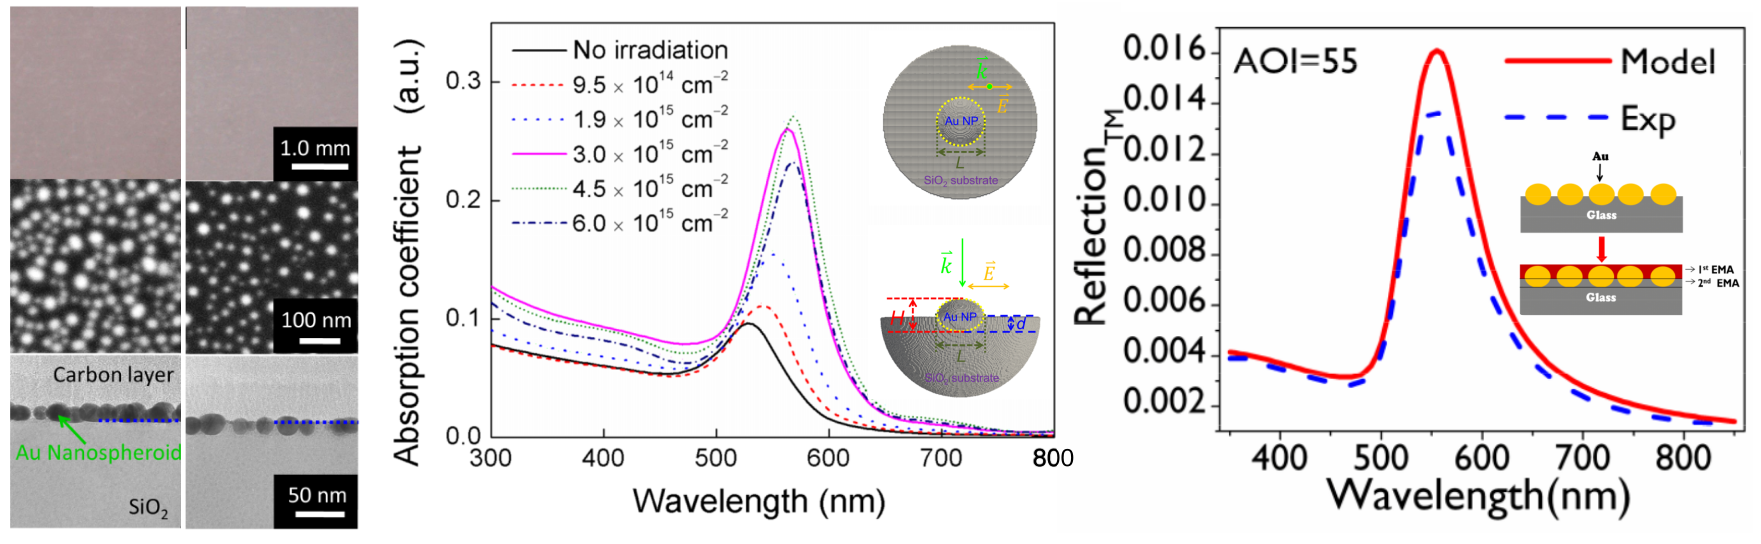
\includegraphics[scale = .7]{embedding.png}};
%
%         \node at (-5.35,1.45) {\ding{172}}; %1
%         \node at (1.25,1.35) {\ding{173}};   %2
%     \end{tikzpicture}
%     \end{center}
%
%     \vspace*{0em}
%         \noindent\rule{.25\textwidth}{0.4pt}
%          \begin{spacing}{0}\fontsize{4}{12} \selectfont
%             $^1$ \fullcite{meng_anisotropic_2015}\\
%             $^2$ \fullcite{moirangthem_enhanced_2012}
%          \end{spacing}
% \end{frame}


%----------------------------------------------------------------------------------
\begin{frame}{Objetivo}{Estudio del incrustamiento parcial de meta-átomos en el sustrato}
   \begin{center}
  	\begin{tikzpicture}[node distance=1em and 1em,font=\small]
        \path (-7.5,0) node [flowbox] (bio) {\fbtitle{Incrustamiento de meta-átomos}\vphantom{yÖ}
	    \nodepart{two}
         \begin{minipage}{.3\textwidth}
         \begin{itemize}%[<+->]
         \item Proceso de fabricación$^1$
         \item Característica deseable para biosensado
            \begin{itemize}
            \item Acoplamiento con  sistemas de microfluídica
            \end{itemize}
         \item \textbf{¿Detección óptica?}
        \end{itemize}\end{minipage}
        };
%
         \node at (0,-1.5) {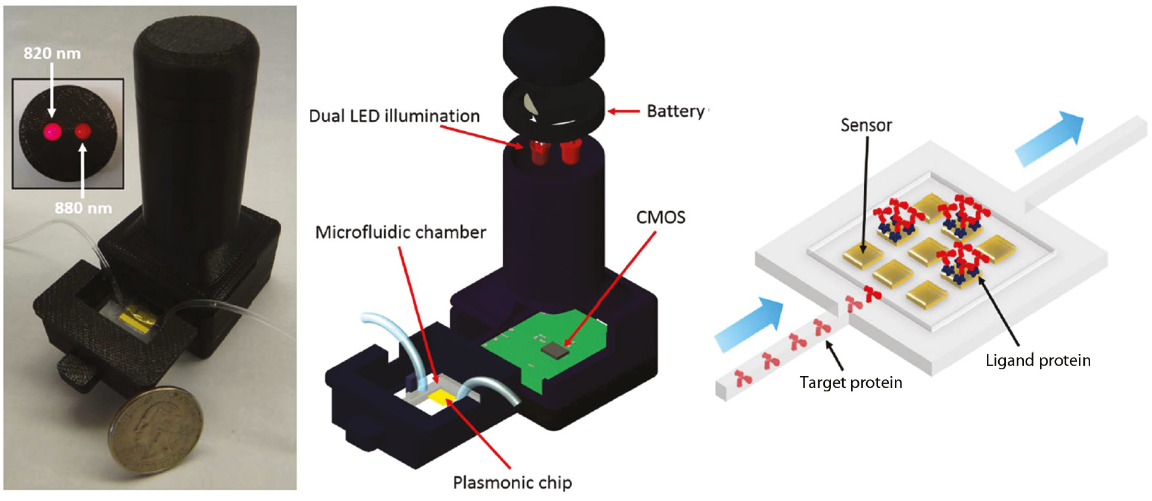
\includegraphics[scale = .3, trim = {0 0 0 0}, clip]{micro.png}};

         \node at (0,+1.5) {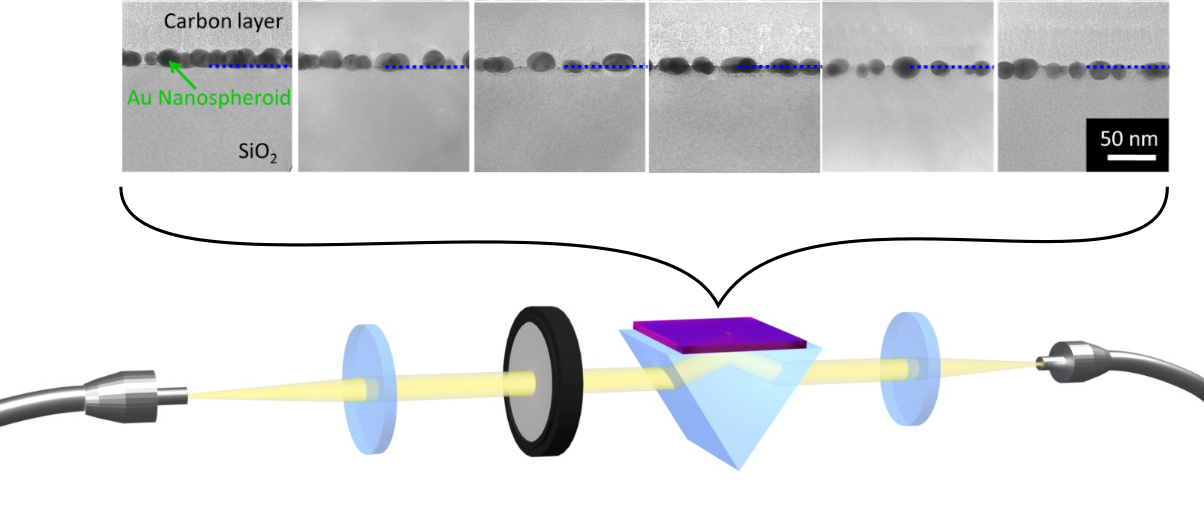
\includegraphics[scale = 1.05, trim = {30 80 10 0}, clip]{exp-NPs.png}};
    \end{tikzpicture}
\end{center}

    \vspace*{0em}
        \noindent\rule{.25\textwidth}{0.4pt}
         \begin{spacing}{0}\fontsize{4}{12} \selectfont
            $^1$ \fullcite{meng_anisotropic_2015}\\
            $^2$ \fullcite{moirangthem_enhanced_2012}
         \end{spacing}
\end{frame}


%----------------------------------------------------------------------------------
\begin{frame}{Sistema de interés}{Meta-átomo: Nanopartíula (NP) esférica de oro (Au) apta para biosensado}

      \begin{center}
  	\begin{tikzpicture}[node distance=1em and 1em,font=\small]
        \path (-7.5,-1) node [flowbox] (bio) {\fbtitle{FC-UNAM$^1$ -- INAOE$^{2}$}\vphantom{yÖ}
	    \nodepart{two}
         \begin{minipage}{.35\textwidth}
          Desarrollo de un biosensor plasmónico:\\

          \begin{itemize}
            \item Colaboración teórico-experimental
			\item Metasuperficie desordenada
            \item Mediciones de reflectancia
%                \begin{itemize}
%                   \item Polarización $s$
%                   \item Polarización $p$
%                \end{itemize}
% 			\item Incidencia oblicua
         \end{itemize}\end{minipage}
        };

        \node at (-2.25,-0.25) {Esquema del sistema experimental$^3$:};
          \node at (0,-1.75) {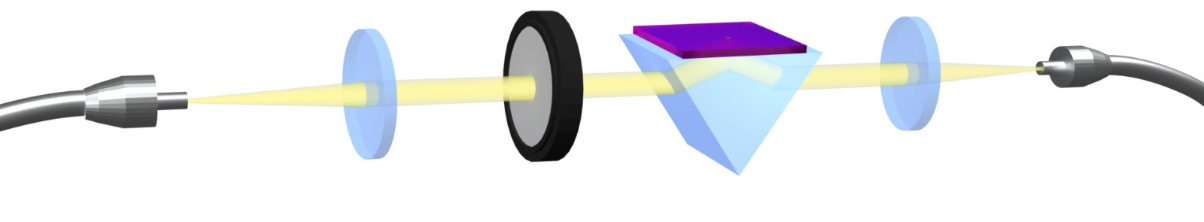
\includegraphics[scale = .8]{sistExp.png}};

        \node at (-3,-0.75) {\footnotesize Fuente de luz blanca};
        \node at (1.,-0.75) {\footnotesize Muestra sobre prisma};
        \node at (3.5,-0.75) {\footnotesize Detector};

        \node at (-1.6,-2.5) {\footnotesize Lente};
        \node at (-.25,-2.5) {\footnotesize Polarizador};
        \node at (2.1,-2.5) {\footnotesize Lente};

        \path (-7.5,-4) node [flowbox] (bio) {\fbtitle{Meta-átomo:}\vphantom{yÖ}
	    \nodepart{two}
         \begin{minipage}{.25\textwidth}
          \begin{itemize}
			\item AuNP esférica
            \item Radio $a$: 12.5 nm
			\item Matriz: Aire
			\item Sustrato: Vidrio
			\item Incrustamiento parcial
         \end{itemize}\end{minipage}
        };

        \node at (0,-4.75) {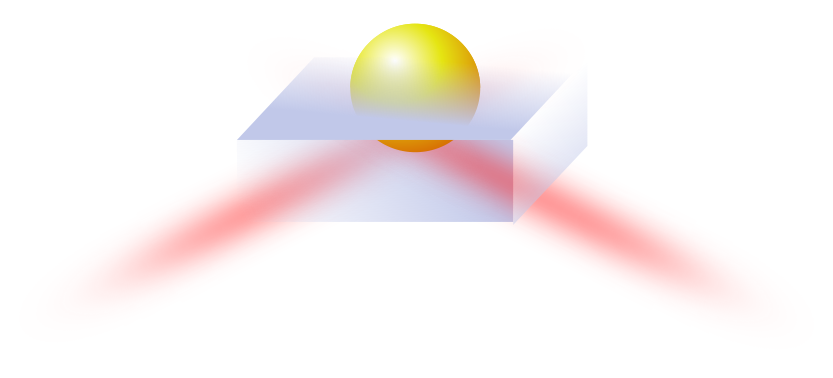
\includegraphics[scale = 1.1]{NP.png}};
        \node at (-3,-3.0) {Esquema del meta-átomo:};

        \node at (1,-3.5) {\footnotesize Matriz};
        \node at (.5,-4.75) {\footnotesize Sustrato};

    \end{tikzpicture}
    \end{center}

    \vspace*{-3.5em}
        \noindent\rule{.25\textwidth}{0.4pt}
         \begin{spacing}{0}\fontsize{4}{12} \selectfont
            $^1$ Grupo de Nanoplasmónica\\
            $^2$ Grupo de Biofotónica y Grupo de Optoelectrónica de semiconductores orgánicos e híbridos\\
            $^3$ Esquema realizado Juan Pablo Cuanalo Fernández.
         \end{spacing}
\end{frame}


\begin{frame}{Contenido}\label{fr:Contenido}
\vfill
\begin{columns}
\column{.5\textwidth}
    \tableofcontents
\column{.5\textwidth}
    \hspace*{-3em}\begin{tikzpicture}[node distance=1em and 1em]
        \path (1,0) node {
            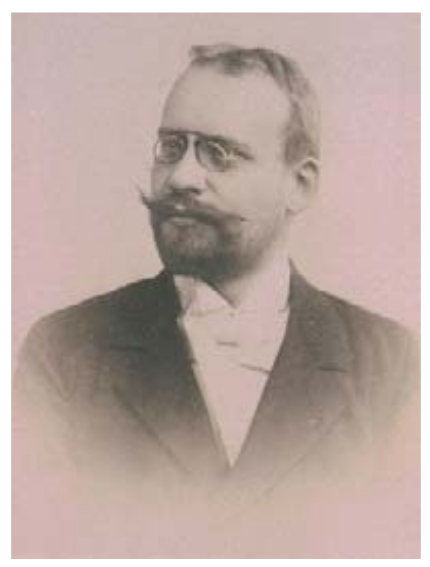
\includegraphics[scale = .3]{Mie.png}
        };
        %
      \path (-1.5,1.65) node {\begin{minipage}{.18\textwidth}
                        \tiny
                         Fotografía de Gustav Mie alrededor de 1905$^1$
                         \end{minipage}
                         };
      \path (-3.95,-2.25) node {
%             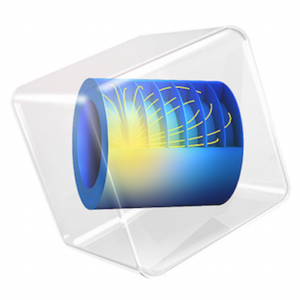
\includegraphics[scale = .3]{comsol.png}
            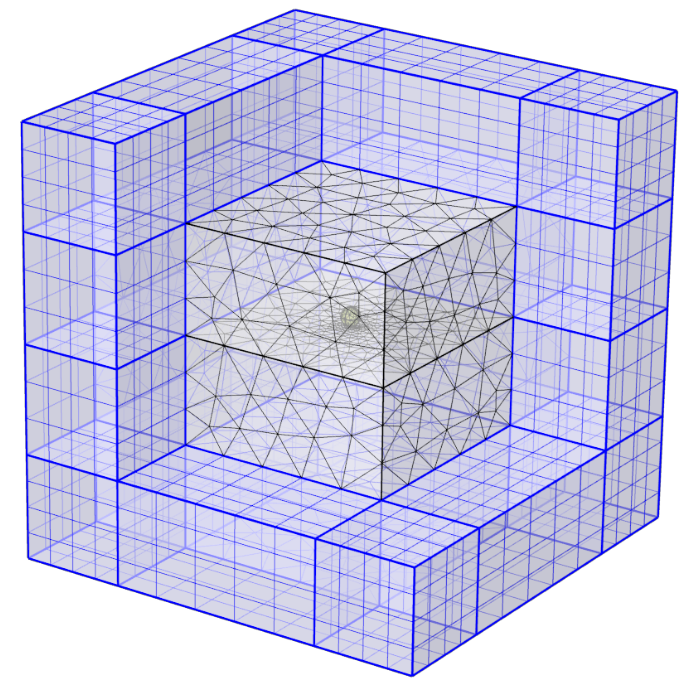
\includegraphics[scale = .15]{Geometries/sist.png}
        };
        %
      \path (-1.5,-3.5) node {\begin{minipage}{.5\textwidth}
                        \tiny
                         COMSOL Multiphysics\textsuperscript{\texttrademark} Ver. 5.4
                         \end{minipage}
                         };
    \end{tikzpicture}
\end{columns}
\vfill
\noindent\rule{.25\textwidth}{0.4pt}
         \begin{spacing}{0}\fontsize{4}{12} \selectfont
            $^1$ \fullcite{horvath_gustav_2009}
         \end{spacing}
\end{frame}




\section{Teoría}
\subsection{Esparcimiento por una partícula esférica}

\begin{frame}{Esparcimiento por una partícula}{Secciones transversales de absorción, esparcimiento y extinción}
    \begin{columns}
	\column{.45\textwidth}\centering \small
	\tdplotsetmaincoords{60}{110}
 \pgfmathsetmacro{\rvec}{1. 3}
 \pgfmathsetmacro{\thetavec}{30}
 \pgfmathsetmacro{\varphivec}{60}
\begin{tikzpicture}[scale=2.7,tdplot_main_coords]
 %draw the NP
 %\draw[tdplot_screen_coords,ball color=yellow, opacity = 1] (0,0,0) circle (.05);
 %\draw[tdplot_screen_coords, color=yellow, opacity = 1] (0,0,0) circle (.05);

 \pgfmathsetseed{3}
     \draw[tdplot_screen_coords, ball color=yellow, opacity = 1,scale =.075]
     plot [smooth cycle, samples=8,domain={1:8}]
         (\x*360/8+5*rnd:0.5cm+1cm*rnd) node at (0,0) {};
 \pgfmathsetseed{3}
     \draw[tdplot_screen_coords, color=yellow, opacity = 1,scale =.075]
      plot [smooth cycle, samples=8,domain={1:8}]
      (\x*360/8+5*rnd:0.5cm+1cm*rnd) node at (0,0) {};


 % Set up some coordinates
  \coordinate (O) at (0,0,0);

 %determine a coordinate (P) using (r,\theta,\varphi) coordinates.   This command
 %also determines (Pxy), (Pxz), and (Pyz): the xy-, xz-, and yz-projections
 %of the point (P).
 %syntax: \tdplotsetcoord{Coordinate name without parentheses}{r}{\theta}{\varphi}
 \tdplotsetcoord{P}{\rvec}{\thetavec}{\varphivec}

 %draw figure contents
 %--------------------
 %draw the main coordinate system axes
     \draw[thick,- latex] (0,0,0) -- (1. 5,0,0) node[anchor=north east]{$x$};
     \draw[thick,- latex] (0,0,0) -- (0,1. 5,0) node[anchor=north west]{$y$};
     \draw[thick,- latex] (0,0,0) -- (0,0,1. 5) node[anchor=south]{$z$};

 %draw the main cartesian vector system
     \draw[thick,- latex, blue] (0,0,0) -- (1,0,0) node[anchor= south east]{$\vu{e}_x$};
     \draw[thick,- latex, blue] (0,0,0) -- (0,1,0) node[anchor=north west]{$\vu{e}_y$};
     \draw[thick,- latex, blue] (0,0,0) -- (0,0,1) node[anchor= east]{$\vu{e}_z$};

 %draw a vector from origin to point (P)
     \draw[thick,color=green, - latex] (O) -- (P);
     \node at (1,. 5,1. 1) {\color{green} $\vb{r}$};

 %draw projection on xy plane, and a connecting line
     \draw[dashed, color=green] (O) -- (Pxy);
     \draw[dashed, color=green] (P) -- (Pxy);
     \fill[green, opacity = .3] (O) --(Pxy)-- (P)--(O);
     \draw[- latex, tdplot_screen_coords,green](.42,.2)--(.8,.2);
     \node[tdplot_screen_coords] at (1.1,.2) {\begin{minipage}{2.cm}\centering\small \color{green}Plano de esparcimiento\end{minipage} };


 %draw the angle \varphi, and label it
     %syntax: \tdplotdrawarc[coordinate frame, draw options]{center point}{r}{angle}{label options}{label}
     \tdplotdrawarc[- latex]{(O)}{0. 5}{0}{\varphivec}{anchor=south}{$\varphi$}


 %set the rotated coordinate system so the x'-y' plane lies within the
     %"theta plane" of the main coordinate system
     %syntax: \tdplotsetthetaplanecoords{\varphi}
     \tdplotsetthetaplanecoords{\varphivec}

 %draw theta arc and label, using rotated coordinate system
     \tdplotdrawarc[tdplot_rotated_coords, - latex]{(0,0,0)}{0. 45}{0}{\thetavec}{anchor=north}{$\theta$}

 %draw some dashed arcs, demonstrating direct arc drawing
     \draw[dashed,tdplot_rotated_coords] (\rvec,0,0) arc (0:90:\rvec);
     \draw[dashed] (\rvec,0,0) arc (0:90:\rvec);

 %set the rotated coordinate definition within display using a translation
 %coordinate and Euler angles in the "z(\alpha)y(\beta)z(\gamma)" euler rotation convention
 %syntax: \tdplotsetrotatedcoords{\alpha}{\beta}{\gamma}
     \tdplotsetrotatedcoords{\varphivec}{\thetavec}{0}

 %translate the rotated coordinate system
 %syntax: \tdplotsetrotatedcoordsorigin{point}
     \tdplotsetrotatedcoordsorigin{(P)}

 %use the tdplot_rotated_coords style to work in the rotated, translated coordinate frame
     \draw[thick,tdplot_rotated_coords,- latex, purple] (0,0,0) -- (. 3,0,0) node[anchor=north west]{{\color{black}$\vu{e}_\theta,$}$\vu{e}_{\parallel}^\text{sca}$};
     \draw[thick,tdplot_rotated_coords,- latex,black] (0,0,0) -- (0,. 3,0) node[anchor=west]{$\vu{e}_\varphi$};
     \draw[thick,tdplot_rotated_coords,- latex,purple] (0,0,0) -- (0,-. 3,0) node[anchor= north west]{$\vu{e}_{\perp}^\text{sca}$};
     \draw[thick,tdplot_rotated_coords,- latex] (0,0,0) -- (0,0,. 3) node[anchor=south]{$\vu{k}^\text{sca}, \vu{e}_r$ };

 %set the rotated coordinate definition within display using a translation
 %coordinate and Euler angles in the "z(\alpha)y(\beta)z(\gamma)" euler rotation convention
 %syntax: \tdplotsetrotatedcoords{\alpha}{\beta}{\gamma}
     \tdplotsetrotatedcoords{\varphivec}{0}{0}

 %translate the rotated coordinate system
 %syntax: \tdplotsetrotatedcoordsorigin{point}
     \tdplotsetrotatedcoordsorigin{(Pxy)}

     \draw[thick,tdplot_rotated_coords,- latex, purple] (0,0,0) -- (. 3,0,0) node[anchor= west]{$\vu{e}_{\parallel}^\text{i}$};
     \draw[thick,tdplot_rotated_coords,- latex, blue] (0,0,0) -- (0,0,. 3) node[anchor= west]{$\vu{e}_z$};
     \draw[thick,tdplot_rotated_coords,- latex, purple] (0,0,0) -- (0,-. 3,0) node[anchor= north west]{$\vu{e}_{\perp}^\text{i}$};

 % plane wave
     \foreach \i in {-5}{ %{-7,...,-2}{
         \draw[thick,tdplot_screen_coords,red, - latex] (\i/10,0,0)--(\i/10,1,0);}
     \node[tdplot_screen_coords] at (-4.75/10,1.1,0){\color{red}$\vb{k}^\text{i}$};
     \node[tdplot_screen_coords] at (-4.5/10,-.15,0){\begin{minipage}{2.cm}\centering\small \color{red}Onda plana incidente\end{minipage}};
\end{tikzpicture}%

	\column{.55\textwidth}\centering
\begin{alertblock}{Teorema óptico$^1$ y operador de campo lejano$^2$:}	
	
	
 $$ C_\text{ext}  = C_\text{abs} + C_\text{sca} $$
  $$ \vb{E}^\text{sca} =   \frac{\exp(i\vb{k}^\text{sca}\cdot\vb{r})}{r} \mathbb{F}(\vu{k}^\text{sca}, \vu{k}^\text{i}) \vb{E}^\text{i} $$

 \begin{align*}
 C_\text{abs} =&  \frac12\int_\mathcal{V} \frac{\Re(\vb{J}\cdot \vb{E}^\text{int*})}
 									{\norm{\vb{E}_0^\text{i}}^2/2Z_\text{mat}}\dd{V}
 			= \int_\mathcal{V} \omega Z_\text{mat}\Im(n_\text{p}^2) \frac{\norm{\vb{E}^\text{int}}^2}{\norm{\vb{E}^\text{i}_0}^2} \dd{V}\\
 	C_\text{sca} =& \frac{2Z_\text{mat}}{\norm{\vb{E}_0}^2} \oint_\mathcal{S} \ev{\vb{S}^\text{sca}}_t \cdot\dd{\vb{a}}
 	 =  \oint_\mathcal{S} \frac{\norm{\mathbb{F}(\vu{k}^\text{sca},\vu{k}^\text{i})\vb{E}^\text{i}}^2}
									{\norm{\vb{E}^\text{i}_0}^2}\dd{a}\\
C_\text{ext} =&  \frac{4\pi}{k \norm{\vb{E}_0^\text{i}}^2}\Im\qty[ \vb{E}_0^\text{i}\cdot \mathbb{F}^*(\vu{k}^\text{i},\vu{k}^\text{i}) \vb{E}^\text{i*} ]
 \end{align*}
 \end{alertblock}
\end{columns}

\vspace*{2em}
	\noindent\rule{.25\textwidth}{0.4pt}
 \begin{spacing}{0}\fontsize{4}{12} \selectfont
	$^1$ \fullcite{bohren_absorption_1983}\\
	$^2$ \fullcite{tsang_scattering_2000}
	\end{spacing}

  \end{frame}




\begin{frame}{Solución de Mie$^{1,2}$}
	{Esparcimiento por partículas esféricas embebidas en medios infinitos}
	\scriptsize
	\renewcommand{\newcirc}{{\scaleobj{.625}{\circ}}}
\vspace*{-2em}
% 	$$\vb{E}^\text{i} (\vb{r})= E_0 \sum_{\ell = 1}^\infty\frac{i^\ell(2\ell+1)}{\ell(\ell+1)}\qty( \vb{M}_{o1\ell}^{(1)} -i \vb{N}_{e1\ell}^{(1)})
% 	\qquad\qquad
% 	\vb{E}^\text{sca} (\vb{r}) = E_0 \sum_{\ell = 1}^\infty\frac{i^\ell(2\ell+1)}{\ell(\ell+1)}\qty(i a_\ell \vb{N}_{e1\ell}^{(3)} -b_\ell \vb{M}_{o1\ell}^{(3)})
% 	$$
% 	\vspace*{-2em}
	\begin{columns}
	\column{.5\textwidth} \scriptsize
	\begin{align*}
	\vb{E}^\text{i} (\vb{r}) &= E_0 \sum_{\ell = 1}^\infty\frac{i^\ell(2\ell+1)}{\ell(\ell+1)}\qty( \vb{M}_{o1\ell}^{(1)} -i \vb{N}_{e1\ell}^{(1)})\\
	\vb{E}^\text{sca} (\vb{r}) &= E_0 \sum_{\ell = 1}^\infty\frac{i^\ell(2\ell+1)}{\ell(\ell+1)}\qty(i a_\ell \vb{N}_{e1\ell}^{(3)} -b_\ell \vb{M}_{o1\ell}^{(3)})
	\end{align*}

	\begin{figure}
	    \fontsize{4}{5}\selectfont \hfill %
    $\vb{E}^\text{sca} \sim  i a_1 \vb{N}^{(3)}_{\text{e}11}$\hfill
    $\vb{E}^\text{sca} \sim  - b_1 \vb{M}^{(3)}_{\text{o}11}$\hfill
    $\vb{E}^\text{sca} \sim  i a_2 \vb{N}^{(3)}_{\text{e}12}$\hfill
    $\vb{E}^\text{sca} \sim  - b_2 \vb{M}^{(3)}_{\text{o}12}$\hfill\\[-2em]
	\def\svgwidth{1\textwidth}
	\includeinkscape{VSH/P3-VSH}
\end{figure}
\scriptsize
$$ \mathbb{F}(\vu{k}^\text{sca},\vu{k}^\text{i})
            = \mqty(\dfrac{i}{k}S_2(\theta) & 0 \\
			0 & \dfrac{i}{k}S_1(\theta)  )$$
			\vspace*{-2.em}
\begin{align*}
S_1(\theta)  &= \sum_{\ell = 1}^\infty \frac{2\ell+1}{\ell(\ell+1)}
						[a_\ell\tau_\ell(\cos\theta)+b_\ell\pi_\ell(\cos\theta)]
\\
S_2(\theta) &= \sum_{\ell = 1}^\infty \frac{2\ell+1}{\ell(\ell+1)}
						[a_\ell\pi_\ell(\cos\theta)+b_\ell\tau_\ell(\cos\theta)]
\end{align*}

	 	\column{.5\textwidth} \centering
\begin{figure}
	\def\svgwidth{1\textwidth} \fontsize{4}{5}\selectfont
  \includeinkscape{Mie-Au/P1-Efficiencies}\\[1em]
  \def\svgwidth{.95\textwidth} 
	\includeinkscape{Mie-Au/P2-ScatteringMaps}
\end{figure}
	\end{columns}
	\vspace*{.5em}
	\noindent\rule{.25\textwidth}{0.4pt}
 \begin{spacing}{0}\fontsize{4}{5} \selectfont
	$^1$ \fullcite{bohren_absorption_1983}\\
	$^2$ \fullcite{tsang_scattering_2000}
	\end{spacing}
\end{frame}

% !TeX root = ../presentacion.tex


\subsection{Método de elemento finito}

\begin{frame}{Problema de valores propios de Maxwell}{Formulación fuerte y débil del problema de esparcimiento de luz en un volumen $\Omega$}
\small
\begin{alertblock}{\textbf{Formulación fuerte$^1$:} Ecuación diferencial}
				\begin{align*}
					 \nabla \times \qty[\mu^{-1} \nabla \times \vb{E}] - \kappa^2 \vb{E} = \vb{0},
        \qquad
        \text{donde}
        \qquad
        \kappa^2 = (i\omega\sigma +\omega^2 \varepsilon)
    \end{align*}
        \begin{itemize}%[<+->]
         \item  Condiciones de frontera de Dirichlet (D) y de Neumann (N)\vspace*{-.5em}	
    \begin{align*}
    \vu{n}\times \vb{E}(\vb{r})\eval_{\partial \Omega} = \vb{E}_\text{D}
        \qquad\qquad
    \mu^{-1} \nabla \times \vb{E} \times \vu{n} \eval_{\partial \Omega} =  \vb{E}_\text{N}
					\end{align*}
			\end{itemize}
		\end{alertblock}
	
	\begin{alertblock}{\textbf{Formulación  débil$^{1,2}$:} Ecuación integral con el uso de la función de prueba $\boldsymbol{\eta}(\vb{r})$}
        \begin{itemize}%[<+->]
         \item Simplificación mediante integración por partes y teorema de Gauss
					\begin{align*}
					    \int_\Omega \left\{\qty(\mu^{-1}\nabla\times\vb{E})\cdot \qty(\nabla\times\boldsymbol{\eta}) -  \kappa^2  \cdot   \vb{E} \cdot \boldsymbol{\eta} \right\} \dd{\Omega} & - \oint_{\partial\Omega} \qty(\boldsymbol{\eta}\times \vb{E}_\text{N})  \cdot\vu{n}\dd{(\partial\Omega)} = 0
    \end{align*}
    \item Condiciones de frontera \vspace*{-.5em} $$\vu{n}\times \vb{E}(\vb{r})\eval_{\partial \Omega} = \vb{E}_\text{D}.$$
			\end{itemize}
		\end{alertblock}
	
	\noindent\rule{.25\textwidth}{0.4pt}\\    
   \fontsize{4}{5} \selectfont
	$^1$ \fullcite{dhatt_finite_2012}\\
	$^2$ \fullcite{jin_theory_2010}  

\end{frame}

\begin{frame}{Aproximación de elemento finito y método de Galerkin}%
				{Conceptos fundamentales}

   \begin{center}
   
   		$$\text{Sistema de ecuaciones diferenciales en  $\Omega$:}\qquad\mathcal{L}[u(\vb{r})] - {f}_\Omega= {0} \quad	\Longleftrightarrow \quad \int_\Omega \{\mathcal{L}[u(\vb{r})] - {f}_\Omega\}\psi(\vb{r})\dd{\Omega} = 0$$
   
  	\begin{tikzpicture}[node distance=1em and 1em,font=\small]
        \path (0,0) node [flowbox] (fem) {\fbtitle{Elemento finito$^{1-4}$ $\Omega_k$}\vphantom{yÖ}
	    \nodepart{two}
         \begin{minipage}{.28\textwidth} \begin{itemize}
			\item Geometría $$   \bigcup_{k=1}^M \Omega_k = \Omega
        \qquad
    \bigcap_{k=1}^M \Omega_k = \emptyset$$
			\item Espacio de funciones polinomiales $$\{\phi_{i_k}\}_{i_k\leq N_k}$$
			\item Funcional lineal $$\mathcal{F}_{\ell_k}[\phi_{i_k}] = \delta_{{\ell_k}{i_k}}$$
         \end{itemize}\end{minipage}
        };
        
	\node[flowbox,left=of fem] (nodal) {
        \fbtitle{Aproximación nodal$^{1,2}$}\vphantom{yÖ}
    \nodepart{two}
        \begin{minipage}{.28\textwidth}\begin{itemize}
			\item Combinación lineal: $$u(\vb{r}) \approx \sum_i^N u_i \phi_i(\vb{r})$$
			\item Funciones de interpolación : $$\{\phi_{i}\}_{i\leq N}$$
			\item Nodos con valores exactos: $$u_i = u(\vb{r}_i),\;\; \vb{r}_i\in\Omega$$
         \end{itemize}\end{minipage}
    };
    
    	\node[flowbox,right=of fem] (nodal) {
        \fbtitle{Método de Galerkin$^{4}$}\vphantom{yÖ}
    \nodepart{two}
        \begin{minipage}{.30\textwidth}\begin{itemize}
			\item Formulación débil del problema en $\Omega_k$
			\item Funciones de prueba: $$\{\psi_{i_k}\}_{i_k\leq N_k} = \{\phi_{i_k}\}_{i_k\leq N_k}$$
			\item Sistema de ecuaciones algebraicas: $$\mathbb{A} \vb{u} = \vb{f}$$
			donde $A_{i_k j_k} = \int \phi_{i_k}(\vb{r}) \mathcal{L}[\phi_{j_k}(\vb{r})]\dd{\Omega}$, $
				 u_{i_k} = u(\vb{r}_{i_k}) $ y $ f_{j_k} = \int f_{\Omega_k} \phi_{j_k}(\vb{r}) \dd{\Omega}$.
         \end{itemize}\end{minipage}
    };

    \end{tikzpicture}
    \end{center}

	\noindent\rule{.25\textwidth}{0.4pt}\\    
   \fontsize{4}{5} \selectfont
	$^1$ \fullcite{dhatt_finite_2012}\\
	$^2$ \fullcite{larson_finite_2013}\\
	$^3$ \fullcite{jin_theory_2010}\\
	$^4$ \fullcite{fletcher_computational_1984}
\end{frame}


\begin{frame}{Implementación numérica del problema de esparcimiento de luz}{Familia de elementos finitos de Nédélec$^{1,2}$}
\begin{columns}
\column{.5\textwidth}
 \begin{center}
   
  	\begin{tikzpicture}[node distance=1em and 1em,font=\footnotesize]
        \path (0,0) node [flowbox] (fem) {\fbtitle{Aproximación nodal}\vphantom{yÖ}
	    \nodepart{two}
         \begin{minipage}{.28\textwidth}\label{eq:ei} \begin{align*}
{\vb{E}}(\vb{r}) \approx \sum_{i_k} e_{i_k} \boldsymbol{\eta}_{i_k}(\vb{r})
        \qquad
    e_{i} = \vu{t}_{i_k}\cdot \vb{E}(\vb{r}\in E_{i_k})
\end{align*}\end{minipage}
        };
       
    	\node[flowbox,below=of fem] (nodal) {
        \fbtitle{Método de Galerkin}\vphantom{yÖ}
    \nodepart{two}
        \begin{minipage}{.8\textwidth} $$\mathbb{A} \vb{e} = \vb{0}$$ \label{eq:Aij}
        \begin{align*}
    A_{ij}  = &    \int_{\Omega_k} \left\{\qty(\mu^{-1}\nabla\times\boldsymbol{\eta}_i)\cdot\qty(\nabla\times\boldsymbol{\eta}_j)
    			-  \kappa^2  \cdot   \boldsymbol{\eta}_i \cdot \boldsymbol{\eta}_j \right\} \dd{\Omega_k} +\\
    		& - \oint_{\partial\Omega} \qty(\boldsymbol{\eta}_j\times \vb{E}_\text{N}) \cdot\vu{n}\dd{(\partial\Omega)}
\end{align*}\end{minipage}
    };
    
    \node[flowbox,below=of nodal]  {
        \fbtitle{Funcional de Nédélec de menor orden}\vphantom{yÖ}
    \nodepart{two}
        \begin{minipage}{.85\textwidth}
        $$ \mathcal{F}^{N}_{i_k}[\boldsymbol{\eta}_{\ell_k}(\boldsymbol{\xi})] = \frac{1}{\abs{E_{i_k}}}\qty(\int_{E_{i_k}} \vu{t}_{i_k}\cdot\boldsymbol{\eta}_{\ell_k}(\boldsymbol{\xi})   \dd{(\partial\Omega_k)} )^{1/2}  $$\end{minipage}
    };

    \end{tikzpicture}
    \end{center}   

\column{.5\textwidth}\centering
Para geometrías triangulares:
$$\boldsymbol{\eta}_{i_k} = \abs{E_{i_k}} \qty(\phi_{j_k}\nabla\phi_{\ell_k} - \phi_{\ell_k}\nabla\phi_{j_k} )$$
$$\mathcal{F}^{L}_{\ell_k}[\phi_{j_k}(\boldsymbol{\xi})] = \phi_{j_k}(\boldsymbol{\xi}_{\ell_k})$$
\begin{figure}
    \fontsize{4}{5} \selectfont
    \def\svgwidth{1\textwidth}
    \includeinkscape{FEM-Theory/P1-Example-Nedelec}
\end{figure}


\end{columns}
    \vspace*{-.0em}\fontsize{4}{5} \selectfont
   \noindent\rule{.25\textwidth}{0.4pt}\\
	$^1$ \fullcite{jin_theory_2010}\\
	$^2$ \fullcite{larson_finite_2013}
\end{frame}

\subsection{Condiciones de frontera abiertas}
\begin{frame}{Condiciones de frontera abiertas}{Simulando medios infinitos }

\begin{description}
	\item[\textbf{Condición de radiación de Sommerfeld$^1$:}] Comportamiento en el campo lejano 
	$$
    \lim_{r\to\infty} \qty(\vu{e}_r\times\vb{E} - \sqrt{\frac{\mu}{\varepsilon}} \vb{H}) = \lim_{r\to \infty} r\qty(\nabla\times \vb{E} - i k \vu{e}_r\times\vb{E}) = 0  $$
	\item[\textbf{\textit{Perfect Matching Layer$^2$:}}] Película ($\Omega_\text{PML}$) sin impedancia y absorbente basada en su geometría:
	\begin{align*}
	        \left. \mqty{\varepsilon_{{}_\Omega}=\varepsilon_{{}_\text{PML}} ,
                                                &\mu_{{}_\Omega}=\mu_{{}_\text{PML}}
                                                \\
                                                \\
                                            s^{(\Omega)}_x  = s^\text{(PML)}_x,
                                            &  s^{(\Omega)}_y  = s^\text{(PML)}_y} \right\}
                    \qquad\implies \qquad
           r_\text{s} = r_\text{p} = 0 .
\end{align*}	
\end{description} 
\begin{center}
   
  	\begin{tikzpicture}[node distance=1em and 1em,font=\small]
        \path (0,0) node [flowbox] (fem) {\fbtitle{Método de Galerkin$^3$}\vphantom{yÖ}
	    \nodepart{two}
         \begin{minipage}{.28\textwidth}	\begin{align*}
	 \mathbb{A}\vb{e} = \vb{0} \qquad &\text{con}\qquad \text{ con \hyperlink{eq:Aij}{{$\mathbb{A}$} y \hyperlink{eq:ei}{{$\vb{e}$}}  como en la diapositiva anterior,} }\\
         \mathbb{\Lambda} = \text{diag}\qty(s_z, s_z ,s_z^{-1}),      \qquad&\text{con}\qquad     s_z= 1 \text{ en } \Omega \text{ y } \Im[s_z] < 0 \text{ en } \Omega_\text{PML}, \\
         \qty(\mu^{-1}\nabla\times\boldsymbol{\eta}_i)\cdot\qty(\nabla\times\boldsymbol{\eta}_j)   \qquad&\to\qquad   \qty(\mathbb{\Lambda}^{-1}\mu^{-1}\nabla\times\boldsymbol{\eta}_i)\cdot  \qty(\nabla\times\boldsymbol{\eta}_j),\\
         \boldsymbol{\eta}_i \cdot \boldsymbol{\eta}_j  \qquad&\to\qquad  \boldsymbol{\eta}_i \cdot \mathbb{\Lambda} \boldsymbol{\eta}_j.
	\end{align*}\end{minipage}
        };
       
    
    \node[right=of fem]  {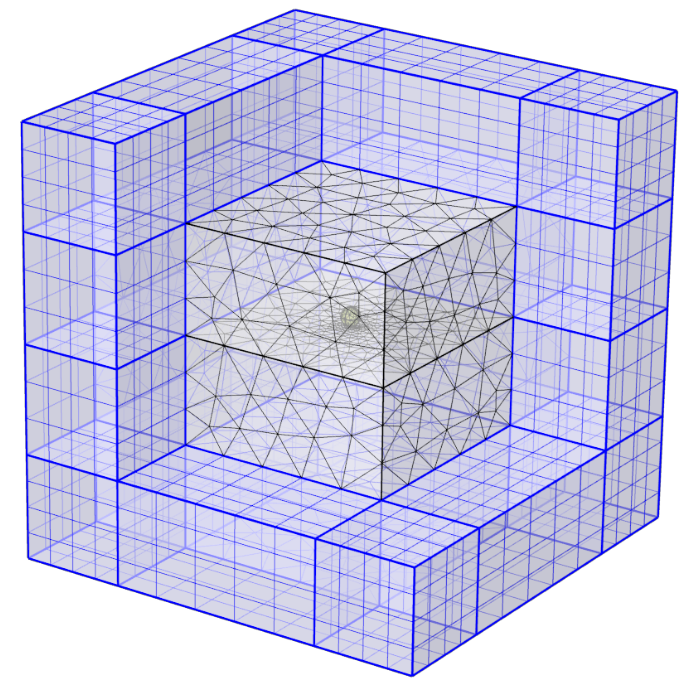
\includegraphics[scale=.2]{Geometries/sist}    };

    \end{tikzpicture}
    \end{center}   
    \vspace*{-1em}\fontsize{4}{5} \selectfont
   \noindent\rule{.25\textwidth}{0.4pt}\\
$^1$ \fullcite{silver_microwave_1984}\\
	$^2$ \fullcite{chew_complex_1997}\\
	$^3$ \fullcite{jin_theory_2010}\\

\end{frame}


































% !TeX root = ../presentacion.tex


\section{Resultados}
% ------------------------------------------------------------------------------------------------------------------
% ------------------------------------------------------------------------------------------------------------------
    \begin{frame}{Análisis de convergencia}{Comsol vs Mie: 12.5 AuNP$@$Aire  y 12.5 AuNP$@$BK7}
    \begin{center}
        \begin{columns}
        \column{.4\textwidth}
      \begin{description}
      \item[\textbf{Tamaño del elemento (matriz):}] $\lambda/(6 n_m)$
      \item[\textbf{Tamaño del elemento (esfera):}] $a/5$
      \item[\textbf{Tamaño de la matriz:}] $2(15+1)an_m$
      \item[\textbf{Grosor PML:}] $\lambda/4$
      \end{description}
        \column{.5\textwidth}\centering\vspace*{-2em}
      \begin{figure}[h!]
        \def\svgwidth{1\textwidth}\footnotesize %\fontsize{4}{5}\selectfont
      \includeinkscape{Geometries/SistemaBox}
    \end{figure}
    \end{columns}
      \begin{figure}[h!]\scriptsize
        \def\svgwidth{.6\textwidth} %\fontsize{4}{5}\selectfont
        \includeinkscape{FEM/4-Conv}
    \end{figure}
    \end{center}
    \end{frame}
% ------------------------------------------------------------------------------------------------------------------
% ------------------------------------------------------------------------------------------------------------------
  \subsection{Esfera soportada y completamente embebida}
  \subsubsection{Incidencia normal}
    \begin{frame}{Esfera soportada y completamente embebida}{Incidencia normal: 12.5 AuNP$@$Aire/BK7}
    \begin{figure}
        \def\svgwidth{.95\textwidth}
        \includeinkscape[pretex = \small]{1-Totally/1-Efficiencies/P1-Normal-Eff}%
    \end{figure}
    \end{frame}
% ------------------------------------------------------------------------------------------------------------------
    \begin{frame}{Esfera soportada y completamente embebida}{Incidencia normal: 12.5 AuNP$@$Aire/BK7}
    \renewcommand{\newcirc}{{\scaleobj{.625}{\circ}}}
    \begin{columns}
    \column{.5\textwidth}
    \begin{figure}    \centering
        \def\svgwidth{.95\textwidth} \fontsize{4}{5}\selectfont
        \includeinkscape{1-Totally/4-5-Far-XY-Embedded/P4-5-Far-XY-Embedded-External}\\[2em]
        %
        \def\svgwidth{.95\textwidth}
        \includeinkscape{1-Totally/4-5-Far-XY-Embedded/P4-5-Far-XY-Embedded-Internal}%
    \end{figure}
    \column{.5\textwidth}
    \begin{figure}\centering
      \def\svgwidth{.95 \textwidth}
      \tiny
      \includeinkscape{1-Totally/2-NearY/P2-NearY-EmbSup}
    \end{figure}
    \end{columns}
    \end{frame}
% ------------------------------------------------------------------------------------------------------------------
\subsubsection{Incidencia oblicua}
    \begin{frame}{Esfera soportada en incidencia interna}{Incidencia oblicua: 12.5 AuNP$@$Aire/BK7}
    \begin{columns}
    \column{.5\textwidth}\renewcommand{\newcirc}{{\scaleobj{.75}{\circ}}}
    \begin{figure}\centering
      \def\svgwidth{1 \textwidth}
      \includeinkscape[pretex = \scriptsize]{2-SuppObl/1-Efficiencies/P1-Oblique-Supp-Eff}
    \end{figure}
    \column{.5\textwidth}\renewcommand{\newcirc}{{\scaleobj{.625}{\circ}}}
    \begin{figure}    \centering \fontsize{4}{5}\selectfont
        \def\svgwidth{1\textwidth}
        \includeinkscape{2-SuppObl/4-5-FarXY/P4-5-Far-XY-S}\\[2em]
        %
        \def\svgwidth{1\textwidth}
        \includeinkscape{2-SuppObl/4-5-FarXY/P4-5-Far-XY-P}%
    \end{figure}
    \end{columns}
    \end{frame}
%
% ------------------------------------------------------------------------------------------------------------------
% ------------------------------------------------------------------------------------------------------------------
  \subsection{Esfera parcialmente incrustada}
    \subsubsection{Incidencia normal}
      \begin{frame}{Esfera parcialmente incrustada}{Incidencia normal: 12.5 AuNP$@$Aire/BK7}
      \renewcommand{\newcirc}{{\scaleobj{.625}{\circ}}}
      \centering
      \begin{columns}
      \column{.5\textwidth}
      \begin{figure}    \centering \fontsize{4}{5}\selectfont
          \def\svgwidth{.96\textwidth}
          \includeinkscape{3-IncNorm/1-Efficiencies/P1-Normal-Eff}\\
      %     %
          \def\svgwidth{.96\textwidth}
          \hspace{.5em}\includeinkscape{3-IncNorm/4-5-FarXY/P4-5-Far-XY}%
      \end{figure}
      \column{.5\textwidth}
      \begin{figure}\centering
        \def\svgwidth{.8\textwidth}\vspace*{-2em} \fontsize{4}{5}\selectfont
        \includeinkscape{3-IncNorm/2-Near/P2-Near}
      \end{figure}
      \end{columns}
      \end{frame}
%
% ------------------------------------------------------------------------------------------------------------------
    \subsubsection{Incidencia oblicua}
      \begin{frame}{Esfera parcialmente incrustada}{Incidencia oblicua: 12.5 AuNP$@$Aire/BK7}
      \vspace{-3.5em}\begin{columns}\scriptsize
      \renewcommand{\newcirc}{{\scaleobj{.85}{\circ}}}
      \column{.4\textwidth}	\begin{table} 

\begin{tabular}{l | r | ccccc} \hline \hline
                                &       & \multicolumn{5}{c}{ $\lambda_\text{res}^\text{abs}$ [nm]}  \\ \hline \hline
                                & $h/a$ & $0^\circ$ & $15^\circ$     & $38^\circ$    & $42^\circ$    & $75^\circ$  \\ \hline
\multirow{9}{*}{\rotatebox{90}{\emph{s} Polarization}}
    & 1.00  & \cellcolor{white!92!gray}510    & \cellcolor{white!92!gray}510    & \cellcolor{white!92!gray}510    & \cellcolor{white!92!gray}510    & \cellcolor{white!84!gray}512.5  \\
    & 0.75  & \cellcolor{white!76!gray}515    & \cellcolor{white!76!gray}515    & \cellcolor{white!76!gray}515    & \cellcolor{white!76!gray}515    & \cellcolor{white!76!gray}515    \\
    & 0.50  & \cellcolor{white!60!gray}520    & \cellcolor{white!60!gray}520    & \cellcolor{white!60!gray}520    & \cellcolor{white!60!gray}520    & \cellcolor{white!60!gray}520    \\
    & 0.25  & \cellcolor{white!52!gray}522.5  & \cellcolor{white!52!gray}522.5  & \cellcolor{white!52!gray}522.5  & \cellcolor{white!52!gray}522.5  & \cellcolor{white!52!gray}522.5  \\
    & 0.00  & \cellcolor{white!44!gray}525    & \cellcolor{white!44!gray}525    & \cellcolor{white!44!gray}525    & \cellcolor{white!44!gray}525    & \cellcolor{white!44!gray}525    \\
    & -0.25 & \cellcolor{white!28!gray}527    & \cellcolor{white!28!gray}527    & \cellcolor{white!28!gray}527    & \cellcolor{white!28!gray}527    & \cellcolor{white!28!gray}527    \\
    & -0.50 & \cellcolor{white!12!gray}530    & \cellcolor{white!12!gray}530    & \cellcolor{white!12!gray}530    & \cellcolor{white!12!gray}530    & \cellcolor{white!12!gray}530    \\
    & -0.75 & \cellcolor{white!12!gray}530    & \cellcolor{white!12!gray}530    & \cellcolor{white!12!gray}530    & \cellcolor{white!12!gray}530    & \cellcolor{white!12!gray}530    \\
    & -1.00 & \cellcolor{white!8!gray}532.5   & \cellcolor{white!8!gray}532.5   & \cellcolor{white!8!gray}532.5   & \cellcolor{white!8!gray}532.5   & \cellcolor{white!8!gray}532.5   \\
\hline\hline
\multirow{9}{*}{\rotatebox{90}{\emph{p} Polarization}}
    & 1.00  & \cellcolor{white!92!gray}510    & \cellcolor{white!84!gray}512.5  & \cellcolor{white!84!gray}512.5  & \cellcolor{white!84!gray}512.5  & \cellcolor{white!84!gray}512.5  \\
    & 0.75  & \cellcolor{white!76!gray}515    & \cellcolor{white!76!gray}515    & \cellcolor{white!68!gray}517.5  & \cellcolor{white!68!gray}517.5  & \cellcolor{white!68!gray}517.5  \\
    & 0.50  & \cellcolor{white!60!gray}520    & \cellcolor{white!60!gray}520    & \cellcolor{white!68!gray}517.5  & \cellcolor{white!68!gray}517.5  & \cellcolor{white!60!gray}520    \\
    & 0.25  & \cellcolor{white!52!gray}522.5  & \cellcolor{white!36!gray}525.5  & \cellcolor{white!60!gray}520    & \cellcolor{white!68!gray}517.5  & \cellcolor{white!36!gray}525.5  \\
    & 0.00  & \cellcolor{white!44!gray}525    & \cellcolor{white!44!gray}525    & \cellcolor{white!52!gray}522.5  & \cellcolor{white!60!gray}520    & \cellcolor{white!52!gray}522.5  \\
    & -0.25 & \cellcolor{white!28!gray}527    & \cellcolor{white!20!gray}527    & \cellcolor{white!44!gray}525    & \cellcolor{white!52!gray}522.5  & \cellcolor{white!44!gray}525    \\
    & -0.50  & \cellcolor{white!12!gray}530    & \cellcolor{white!12!gray}530    & \cellcolor{white!20!gray}527    & \cellcolor{white!44!gray}525    & \cellcolor{white!20!gray}527    \\
    & -0.75 & \cellcolor{white!12!gray}530    & \cellcolor{white!12!gray}530    & \cellcolor{white!12!gray}530    & \cellcolor{white!20!gray}527    & \cellcolor{white!12!gray}530    \\
    & -1.00 & \cellcolor{white!8!gray}532.5   & \cellcolor{white!8!gray}532.5   & \cellcolor{white!12!gray}530    & \cellcolor{white!12!gray}530    & \cellcolor{white!12!gray}530    \\
\hline\hline
\end{tabular}
\end{table}%\includegraphics[width =\textwidth]{img/3-Resultados/tab}
      \column{.55\textwidth}
      \renewcommand{\newcirc}{{\scaleobj{.625}{\circ}}}
      \begin{figure}\centering\fontsize{4}{5}\selectfont
          \def\svgwidth{.9\textwidth}
          \includeinkscape{4-Inc-Obl/1-Efficiencies/P2-Oblique-Inc-Abs}%
      \end{figure}
      \end{columns}
      \end{frame}
% ------------------------------------------------------------------------------------------------------------------
      \begin{frame}{Esfera parcialmente incrustada}{Incidencia oblicua: 12.5 AuNP$@$Aire/BK7}
      \vspace{-3.5em}\begin{columns}\scriptsize
      \renewcommand{\newcirc}{{\scaleobj{.85}{\circ}}}
      \column{.4\textwidth}	\begin{table} 

\begin{tabular}{l | r | ccccc } \hline \hline
                                &       &  \multicolumn{5}{c}{ $\lambda_\text{res}^\text{sca}$ [nm]}  \\ \hline \hline
                                & $h/a$ & $0^\circ$ & $15^\circ$     & $38^\circ$    & $42^\circ$    & $75^\circ$    \\ \hline
\multirow{9}{*}{\rotatebox{90}{\emph{s} Polarization}}
    & 1.00  &  \cellcolor{white!89!orange}525    & \cellcolor{white!89!orange}525    & \cellcolor{white!89!orange}525    & \cellcolor{white!89!orange}525    & \cellcolor{white!89!orange}525    \\
    & 0.75  &  \cellcolor{white!89!orange}525    & \cellcolor{white!89!orange}525    & \cellcolor{white!89!orange}525    & \cellcolor{white!89!orange}525    & \cellcolor{white!89!orange}525    \\
    & 0.50  &  \cellcolor{white!67!orange}530    & \cellcolor{white!67!orange}530    & \cellcolor{white!67!orange}530    & \cellcolor{white!67!orange}530    & \cellcolor{white!67!orange}530    \\
    & 0.25  &  \cellcolor{white!45!orange}535    & \cellcolor{white!45!orange}535    & \cellcolor{white!45!orange}535    & \cellcolor{white!45!orange}535    & \cellcolor{white!45!orange}535    \\
    & 0.00  &  \cellcolor{white!23!orange}537.5  & \cellcolor{white!23!orange}537.5  & \cellcolor{white!23!orange}537.5  & \cellcolor{white!45!orange}535    & \cellcolor{white!45!orange}535    \\
    & -0.25 &  \cellcolor{white!45!orange}535    & \cellcolor{white!45!orange}535    & \cellcolor{white!45!orange}535    & \cellcolor{white!45!orange}535    & \cellcolor{white!45!orange}535    \\
    & -0.50 &  \cellcolor{white!23!orange}537.5  & \cellcolor{white!23!orange}537.5  & \cellcolor{white!23!orange}537.5  & \cellcolor{white!23!orange}537.5  & \cellcolor{white!23!orange}537.5  \\
    & -0.75 &  \cellcolor{white!12!orange}540    & \cellcolor{white!12!orange}540    & \cellcolor{white!12!orange}540    & \cellcolor{white!12!orange}540    & \cellcolor{white!12!orange}540    \\
    & -1.00 &  \cellcolor{white!1!orange}542.5   & \cellcolor{white!1!orange}542.5   & \cellcolor{white!1!orange}542.5   & \cellcolor{white!1!orange}542.5   & \cellcolor{white!12!orange}540    \\
\hline\hline
\multirow{9}{*}{\rotatebox{90}{\emph{p} Polarization}}
    & 1.00  &  \cellcolor{white!89!orange}525    & \cellcolor{white!89!orange}525    & \cellcolor{white!78!orange}527.5  & \cellcolor{white!78!orange}527.5  & \cellcolor{white!89!orange}525    \\
    & 0.75  &  \cellcolor{white!89!orange}525    & \cellcolor{white!89!orange}525    & \cellcolor{white!78!orange}527.5  & \cellcolor{white!78!orange}527.5  & \cellcolor{white!78!orange}527.5  \\
    & 0.50  &  \cellcolor{white!67!orange}530    & \cellcolor{white!67!orange}530    & \cellcolor{white!67!orange}530    & \cellcolor{white!78!orange}527.5  & \cellcolor{white!67!orange}530    \\
    & 0.25  &  \cellcolor{white!45!orange}535    & \cellcolor{white!45!orange}535    & \cellcolor{white!56!orange}532.5  & \cellcolor{white!56!orange}532.5  & \cellcolor{white!56!orange}532.5  \\
    & 0.00  &  \cellcolor{white!23!orange}537.5  & \cellcolor{white!45!orange}535    & \cellcolor{white!45!orange}535    & \cellcolor{white!45!orange}535    & \cellcolor{white!45!orange}535    \\
    & -0.25 &  \cellcolor{white!45!orange}535    & \cellcolor{white!45!orange}535    & \cellcolor{white!56!orange}532.5  & \cellcolor{white!34!orange}535.5  & \cellcolor{white!23!orange}537.5  \\
    & -0.50  &  \cellcolor{white!23!orange}537.5  & \cellcolor{white!23!orange}537.5  & \cellcolor{white!23!orange}537.5  & \cellcolor{white!45!orange}535    & \cellcolor{white!23!orange}537.5  \\
    & -0.75 &  \cellcolor{white!12!orange}540    & \cellcolor{white!12!orange}540    & \cellcolor{white!12!orange}540    & \cellcolor{white!45!orange}535    & \cellcolor{white!12!orange}540    \\
    & -1.00 &  \cellcolor{white!1!orange}542.5   & \cellcolor{white!1!orange}542.5   & \cellcolor{white!12!orange}540    & \cellcolor{white!23!orange}537.5  & \cellcolor{white!12!orange}540    \\
\hline\hline
\end{tabular}
\end{table}%\includegraphics[width =\textwidth]{img/3-Resultados/tab}
      \column{.55\textwidth}
      \renewcommand{\newcirc}{{\scaleobj{.625}{\circ}}}
      \begin{figure}\centering\fontsize{4}{5}\selectfont
          \def\svgwidth{.9\textwidth}
          \includeinkscape{4-Inc-Obl/1-Efficiencies/P3-Oblique-Inc-Sca}%
      \end{figure}
      \end{columns}
      \end{frame}
% ------------------------------------------------------------------------------------------------------------------
      \begin{frame}{Esfera parcialmente incrustada}{Incidencia oblicua en polarización $p$: 12.5 AuNP$@$Aire/BK7}\fontsize{4.5}{5.5}\selectfont
      \renewcommand{\newcirc}{{\scaleobj{.625}{\circ}}}
      \begin{columns}
      \column{.5\textwidth}	\begin{figure} \centering
          \def\svgwidth{.85\textwidth}
          \includeinkscape{4-Inc-Obl/5-FarXY-P/P4-5-Far-XY-P-15}\\[1em]
          \def\svgwidth{.85\textwidth}
          \includeinkscape{4-Inc-Obl/5-FarXY-P/P4-5-Far-XY-P-38}%
      \end{figure}
      \column{.5\textwidth}	\begin{figure} \centering
          \def\svgwidth{.85\textwidth}
          \includeinkscape{4-Inc-Obl/5-FarXY-P/P4-5-Far-XY-P-42}\\[1em]
          \def\svgwidth{.85\textwidth}
          \includeinkscape{4-Inc-Obl/5-FarXY-P/P4-5-Far-XY-P-75}%
      \end{figure}
      \end{columns}
      \end{frame}
% ------------------------------------------------------------------------------------------------------------------
      \begin{frame}{Esfera parcialmente incrustada}{Incidencia después del ángulo crítico: 12.5 AuNP$@$Aire/BK7}%\fontsize{4}{5}\selectfont
      \renewcommand{\newcirc}{{\scaleobj{.625}{\circ}}}
      \begin{columns}\fontsize{4}{5}\selectfont
      \column{.5\textwidth}	\begin{figure} \centering
          \def\svgwidth{.85\textwidth}
          \includeinkscape{4-Inc-Obl/5-FarXY-P/P4-5-Far-XY-P-42}\\[1em]
          \def\svgwidth{.85\textwidth}
          \includeinkscape{4-Inc-Obl/4-FarXY-S/P4-5-Far-XY-S-42}%
      \end{figure}
      \column{.5\textwidth}
      \renewcommand{\newcirc}{{\scaleobj{.625}{\circ}}}
      \begin{figure}\centering
        \def\svgwidth{.8\textwidth}\vspace*{-2em} \fontsize{4}{5}
          \includeinkscape{4-Inc-Obl/2-Near-SP/P2-NearYX-SP-42-Ver2}%
      \end{figure}
      \end{columns}
      \end{frame}

% ------------------------------------------------------------------------------------------------------------------
% ------------------------------------------------------------------------------------------------------------------
      \begin{frame}{Resumen}%{Incidencia después del ángulo crítico: 12.5 AuNP$@$Aire/BK7}%\fontsize{4}{5}\selectfont
      \begin{center}
  	\begin{tikzpicture}[node distance=1em and 1em,font=\small]
        \path (0,0) node [flowbox] (Sus) {\fbtitle{Efecto del sustrato}\vphantom{yÖ}
	    \nodepart{two}
	    Anisotropía:\\
         \begin{minipage}{.3\textwidth} \begin{itemize}
			\item Campo cercano
            \item Patrón de radiación
         \end{itemize}\end{minipage}
        };

%         \node[below = of Sus] {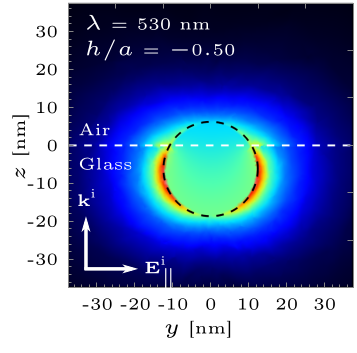
\includegraphics[width = .28\textwidth]{P-Resumen/P1.png}};
          \node[below = of Sus]{\def\svgwidth{.3\textwidth}%
          \fontsize{5}{6}%
          \includeinkscape{P-Resumen/P2-Near}};%}

        \node[flowbox, right = of Sus] (Ilu) {\fbtitle{Efecto de la iluminación}\vphantom{yÖ}
        \nodepart{two}
         \begin{minipage}{.275\textwidth}
          \begin{itemize}
          \item Partícula parcialmente embebida e incidente interna
            \begin{itemize}
            \item Onda plana $\theta_i < \theta_c$
            \item Onda evanescente $\theta_i > \theta_c$
         \end{itemize}
         \item Maximización de propiedads ópticas $\theta_i  \approx \theta_c$
        \end{itemize}
         \end{minipage}
        };

%         \node[below = of Ilu] {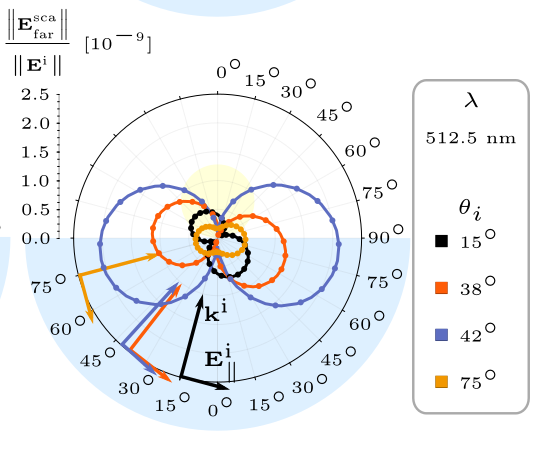
\includegraphics[width = .28\textwidth]{P-Resumen/P2.png}};
          \node[below = of Ilu]{\renewcommand{\newcirc}{{\scaleobj{.7}{\circ}}}%
          \def\svgwidth{.3\textwidth}%
          \fontsize{4.5}{5.5}%
          \includeinkscape{P-Resumen/P4-5-Far-XY-P}};%}

        \node[flowbox, right = of Ilu] (Inc) {\fbtitle{Efecto de la incrustación}\vphantom{yÖ}
        \nodepart{two}
         \begin{minipage}{.3\textwidth}
          \begin{itemize}
            \item Corrimiento al rojo (LSPR)
            \item Aumento de la extinción
            \item Pol. \textit{s}:
            \begin{itemize}
              \item Proceso homogéneo
            \end{itemize}
            \item Pol. \textit{p}:
                        \begin{itemize}
              \item $h/a$ y $\theta_i$
            \end{itemize}
          \end{itemize}\end{minipage}
        };

%         \node[below = of Inc] {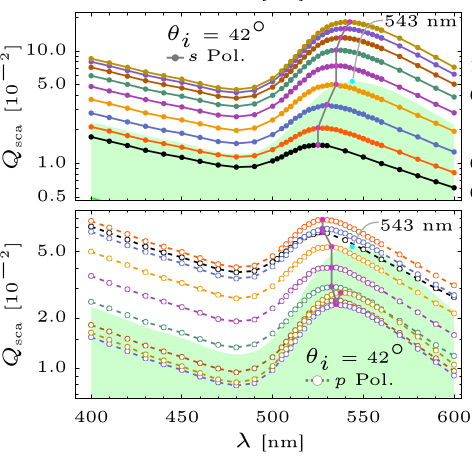
\includegraphics[width = .28\textwidth]{P-Resumen/P3.png}};
          \node[below = of Inc]{\renewcommand{\newcirc}{{\scaleobj{.625}{\circ}}}%
          \def\svgwidth{.275\textwidth}%
          \fontsize{4}{5}%
          \includeinkscape{P-Resumen/P2-Oblique-Inc-Abs}};%}

        \end{tikzpicture}
        \end{center}
      \end{frame}


% !TeX root = ../Avances.tex


\section{Conclusiones y trabajo a futuro}

\begin{frame}{Conclusiones}{Para una AuNP de 12.5 nm de radio parcialmente embebida entre un sustrato plano y una matriz}

  \begin{center}
  	\begin{tikzpicture}[node distance=1em and 1em,font=\small]

        \path (0,0) node [flowbox] (inc) {
        \fbtitle{Incrustación}\vphantom{yÖ}
	    \nodepart{two}
         \begin{minipage}{.28\textwidth}
         A lo más un octavo del  volumen en
         \begin{itemize}
			\item Sustrato $\to$ AuNP soportada
			\item Matriz $\to$ AuNP totalmente embebida
         \end{itemize}
         \end{minipage}
        };


	\node[flowbox,left=of inc] (trans) {
        \fbtitle{Transición}\vphantom{yÖ}
    \nodepart{two}
        \begin{minipage}{.28\textwidth}\begin{itemize}
			\item  Contribución mayormente dipolar
  	\item Transición \textit{suave} entre los dos casos límites de Mie
         \end{itemize}\end{minipage}
    };

    \node[flowbox,right=of inc] (pol) {
        \fbtitle{Iluminación}\vphantom{yÖ}
    \nodepart{two}
        \begin{minipage}{.28\textwidth}
        Resonancia y la distribución espacial del campo eléctrico
        \begin{itemize}
			\item  Pol. $s$:  no dependen de el ángulo de incidencia.
			\item Pol. $p$: sí dependen de el ángulo de incidencia.
         \end{itemize}
         $\theta_i \approx \theta_c$: Máximización de la extinción
		\end{minipage}
    };

    \node[below = of inc]{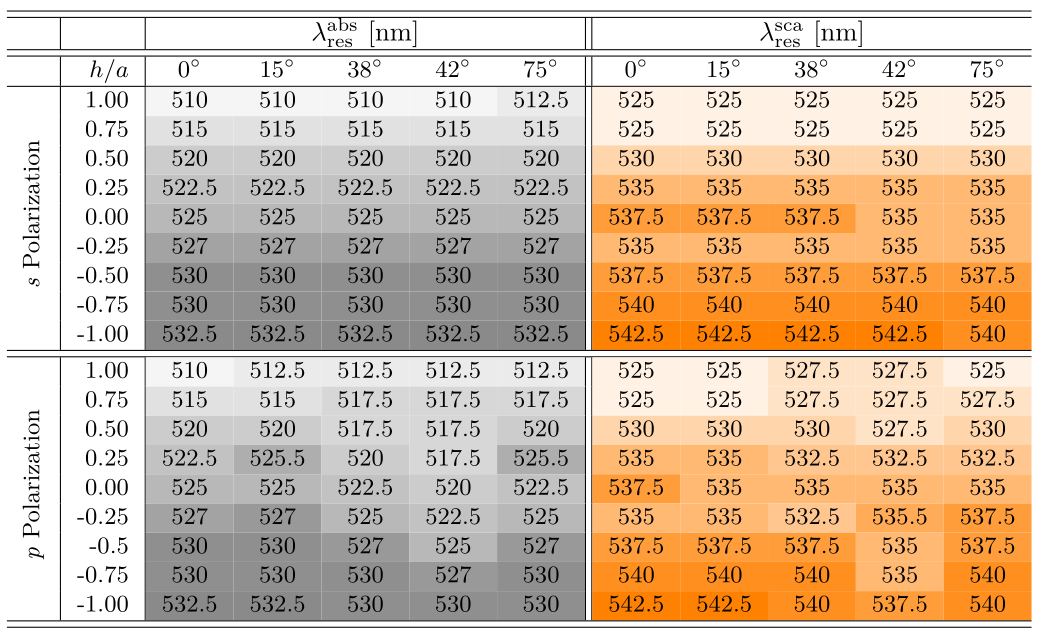
\includegraphics[scale  = .15]{Trans.png}};
    \node[below = of trans]{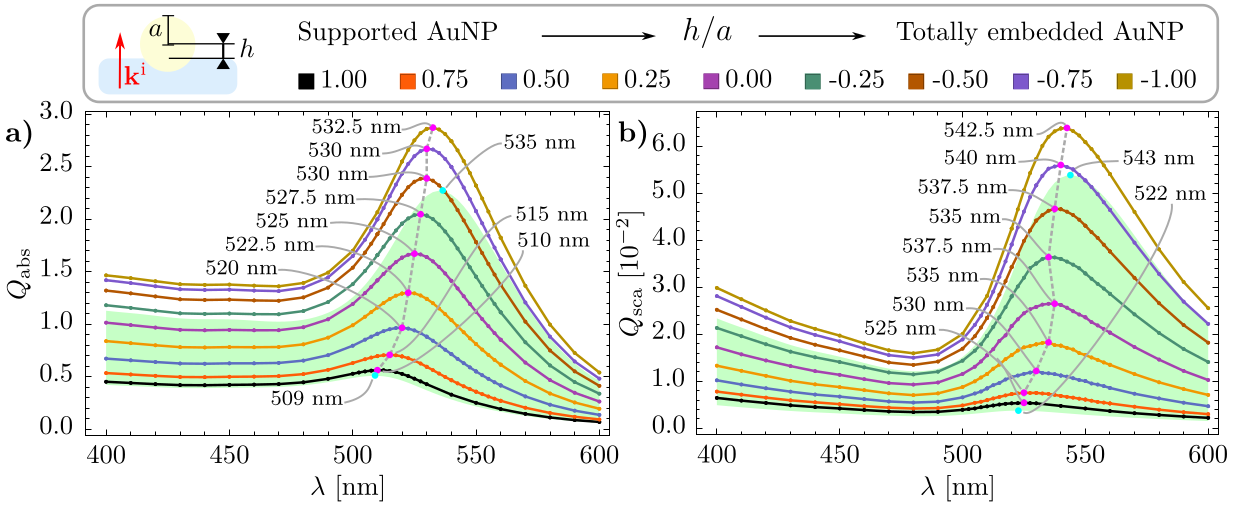
\includegraphics[scale  = .15]{Dip-Mie.png}};
    \node[below = of pol]{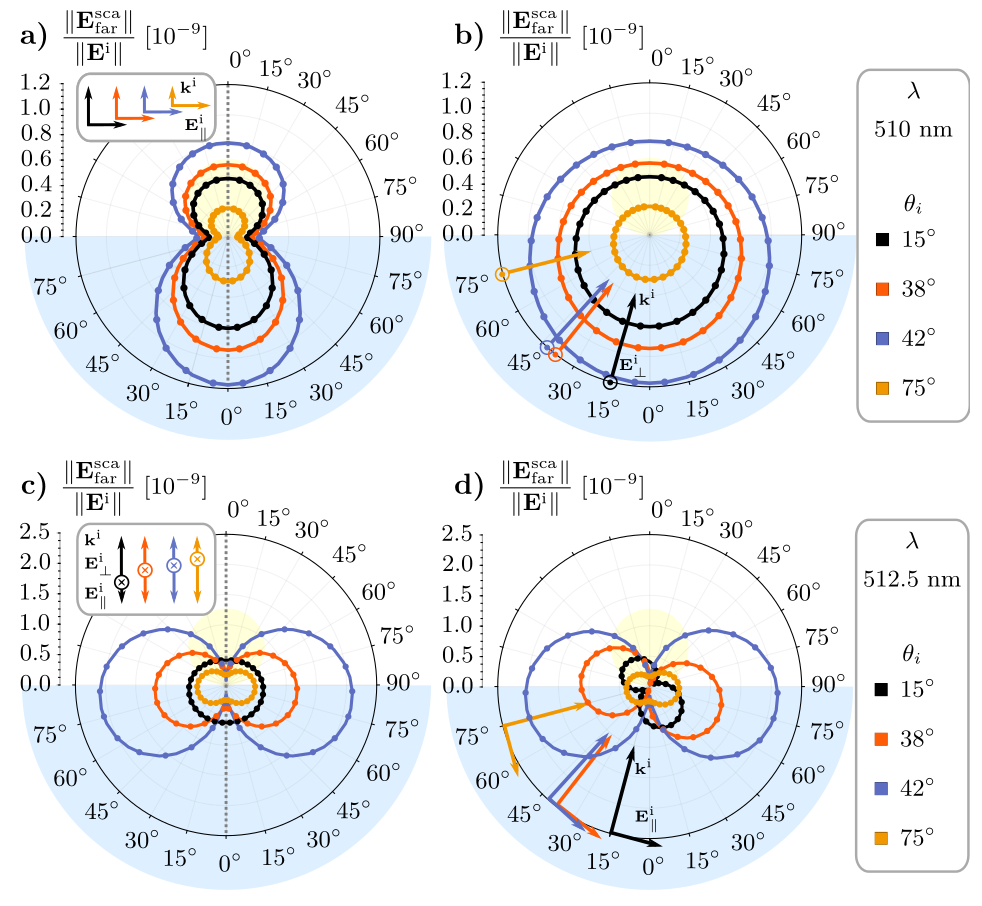
\includegraphics[scale  = .15]{Distribucion.png}};
  \end{tikzpicture}
  \end{center}

\end{frame}



\begin{frame}{Trabajo a futuro}{Para una NP parcialmente embebida entre un sustrato plano y una matriz}

  \begin{center}
  	\begin{tikzpicture}[node distance=1em and 1em]

        \path (0,0) node [flowbox] (meta) {
        \fbtitle{Propiedades ópticas del meta-átomo (Cálculos numéricos)}\vphantom{yÖ}
	    \nodepart{two}
         \begin{minipage}{.85\textwidth}\small
         Determinar secciones transversales como función de la longitud de onda $\lambda$ y polarización de la onda plana que ilumina el sistema, del ángulo de incidencia $\theta_i$ y el grado de incrustación $h/a$ del meta-átomo.
         \end{minipage}
        };

    \path (-3.75,-3) node [flowbox] (eff) {
        \fbtitle{Homogenización + Medio efectivo}\vphantom{yÖ}
	    \nodepart{two}
         \begin{minipage}{.45\textwidth}\small
         Proponer un modelo semi-analítico para la respuesta óptica de una monocapa parcialmente incrustrada:\\

         \begin{itemize}
			\item Homogenización tipo Brüggemman$^1$ del índice de refracción efectivo que envuelve a las NPs.
			\item Empleo de teorías como el Modelo Dipolar$^2$, Teoría de Islas Delgadas$^3$ para la respuesta del sistema monocapa.
         \end{itemize}
         \end{minipage}
        };

    \path (3.75,-3.35) node [flowbox] (exp) {
        \fbtitle{Medición del incrustamiento promedio}\vphantom{yÖ}
	    \nodepart{two}
         \begin{minipage}{.45\textwidth}\small
         Propuesta de un esquema de medición para medir el incrustamiento promedio de la monocapa:\\

         \begin{itemize}
			\item Medición de la $\lambda_{\text{res}}$ para al menos dos valores de $\theta_i>\theta_c$ en ambas polarizaciones.
			\item Comparar el corrimiento de $\lambda_{\text{res}}$ relativo entre ambas polarizaciones.
			\item Con base en las propiedades de un meta-átomo determinar a qué valores de $h/a$ corresponden las mediciones anteriores.
         \end{itemize}
         \end{minipage}
        };

    \draw[- latex, thick] (meta.south) -- (eff.north);
    \draw[- latex, thick] (meta.south) -- (exp.north);
    \end{tikzpicture}
    \end{center}

\noindent\rule{.25\textwidth}{0.4pt}\\
\fontsize{4}{5} \selectfont
	$^1$ \fullcite{sihvola_electromagnetic_2008}\\
	$^2$ \fullcite{barrera1991optical}\\
	$^3$ \fullcite{bedeaux_optical_2004}
\end{frame}


% !TeX root = ../presentation.tex

\begin{frame}{Agradecimientos}{Grupo de Nanoplasmónica, DGAPA, CONACyT, y más...}%{Para una 12.5 nm AuNP parcialmente embebida entre un sustrato plano y una matriz}

 \begin{columns}
 \column{.5\textwidth}
    \centering
    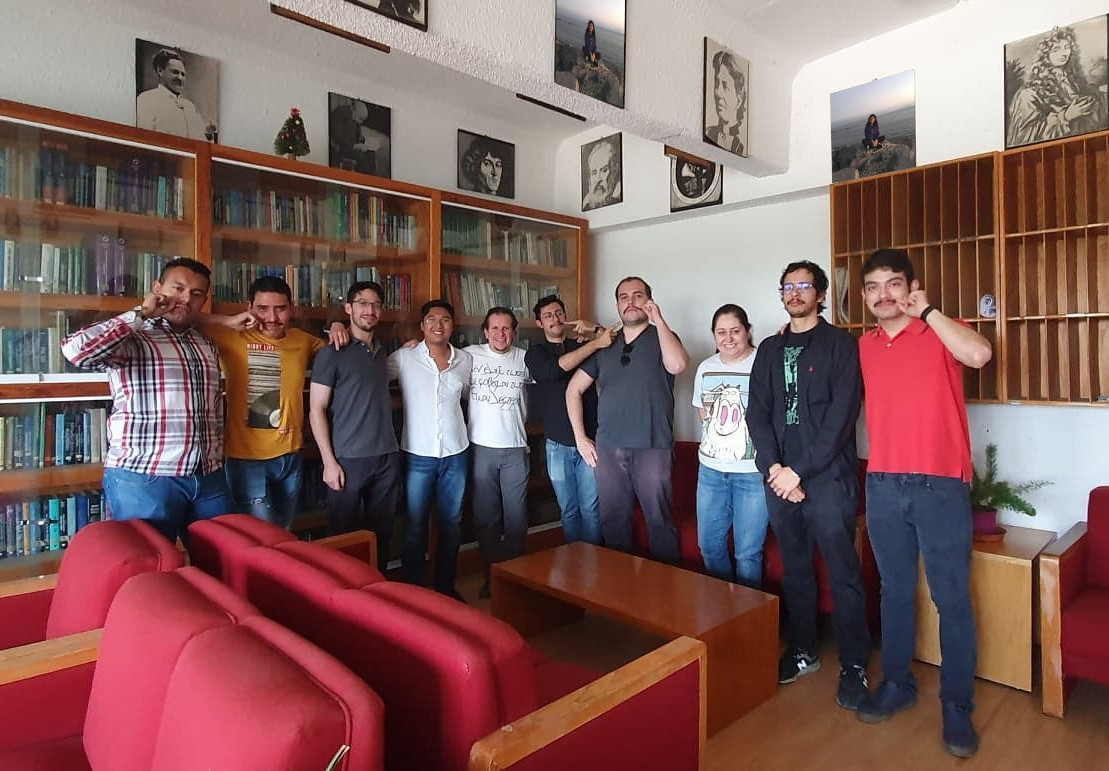
\includegraphics[width = .9\textwidth]{grupo3.jpg}
 \column{.2\textwidth}
 \centering
 \textbf{\large Comité tutor}\\[1em]
       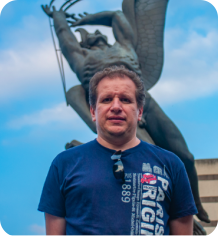
\includegraphics[width = .45\textwidth]{AReyes.png}\\ {\small Dr. Reyes Coronado}\\[.75em]
        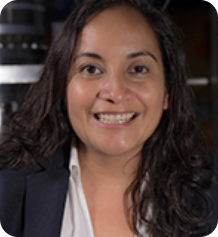
\includegraphics[width = .45\textwidth]{CSanchez.png}\\ {\small Dra. Sánchez Aké}\\[.75em]
         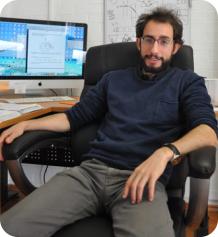
\includegraphics[width = .45\textwidth]{GPirruccio.png}\\ {\small Dr. Pirruccio}
 \column{.3\textwidth}
 \centering
 \includegraphics[width = .6\textwidth]{CONACyT.png}\\[2em]
 
\includegraphics[width = .6\textwidth]{dgapa_unam_azul.png}\\
 {\small PAPIIT IN107122}\\[2em]
 
\includegraphics[width = .4\textwidth]{inaoe.png}
\end{columns}
\end{frame}


\appendix

\begin{frame}{Secciones de apoyo}\label{fr:Apoyo}
    \tableofcontents
\end{frame}

\section{Armónicos esféricos vectoriales}
    

\begin{frame}{Armónicos esféricos vectoriales$^1$: $\{\vb{L},\vb{M}, \vb{N}\}$}
{Base de campos vectoriales que son solución a la ecuación de Helmholtz \hyperlink{fr:Apoyo}{\beamerreturnbutton{}}}\small
\begin{align*}
	\vb{L} = \nabla \psi \qquad \qquad
	\vb{M} = \nabla\times(\vb{r}\psi) \qquad \qquad
	\vb{N} =  \frac{1}{k}\nabla\times\vb{M} \\
	\text{Función generadora }\psi:\,\qquad\nabla^2 \psi + k^2 \psi = 0
\end{align*}%

 Considerando el sistema coordenado esférico:\\[1em]

\begin{columns}
\column{.05\textwidth}
\column{.4\textwidth}
$$ \psi_{ { }^{\text{e}}_{\text{o}}\ell m}(r,\theta,\varphi) =
			\, {\, }^{\sin(m\varphi)}_{\cos(m\varphi)}	P_\ell^m(\cos\theta)z_\ell(kr),$$
 \begin{align*}
 	\vb{L}_{{ }^{\text{e}}_{\text{o}} m\ell} =&
			{\, }^{\cos(m\varphi)}_{\sin(m\varphi)} k P_\ell^m(\cos\theta)\dv{z_\ell(kr)}{(kr)}\,\vu{e}_r
 			+ {\,}^{\cos(m\varphi)}_{\sin(m\varphi)} k\frac{z_\ell(kr)}{kr}\dv{P_\ell^m(\cos\theta)}{\theta} \,\vu{e}_\theta +  \\
			&  {\, }^{-\sin(m\varphi)}_{+\cos(m\varphi)} km \frac{P_\ell^m(\cos\theta)}{\sin\theta}\frac{z_\ell(kr)}{kr} \,\vu{e}_\varphi\\
	\vb{M}_{{ }^{\text{e}}_{\text{o}} m\ell} = &
			{\, }^{-\sin(m\varphi)}_{+\cos(m\varphi)} m z_\ell(kr) \frac{P_\ell^m(\cos\theta)}{\sin\theta}\,\vu{e}_\theta
			-{\, }^{\cos(m\varphi)}_{\sin(m\varphi)} z_\ell(kr) \dv{P_\ell^m(\cos\theta)}{\theta}(\cos\theta)\,\vu{e}_\varphi \\
	\vb{N}_{{ }^{\text{e}}_{\text{o}} m\ell} = &
			{\, }^{\cos(m\varphi)}_{\sin(m\varphi)} \frac{z_\ell(kr)}{kr} \ell(\ell+1)P_\ell^m(\cos\theta)\,\vu{e}_r
			+ {\, }^{\cos(m\varphi)}_{\sin(m\varphi)}  \frac{1}{kr} \dv{[kr\, z_\ell(kr)] }{(kr)}
						\dv{P_\ell^m(\cos\theta)}{\theta}(\cos\theta)\,\vu{e}_\theta +  \\
			&  {\, }^{-\sin(m\varphi)}_{+\cos(m\varphi)} m \frac{1}{kr} \dv{[kr\, z_\ell(kr)] }{(kr)}\frac{P_\ell^m(\cos\theta)}{\sin\theta}
		 \,\vu{e}_\varphi
 \end{align*}
\column{.3\textwidth}
\begin{itemize}
\item[$P_m^\ell$:] Funciones asociadas de Legendre
 \item[$z_\ell$:] Funciones esféricas de Bessel (Hankel)\\[1em]
 \end{itemize}

 Comportamiento asintótico$^2$ de $h^{(1)}_\ell= j_\ell + i y_\ell$:
\begin{align*}
	h_\ell^{(1)}(\rho)\approx (-i)^\ell \frac{\exp(i\rho)}{i\rho}
	\\
	\dv{h_\ell^{(1)}(\rho)}{\rho} \approx (-i)^\ell \frac{\exp(i\rho)}{\rho},
\end{align*}
\column{.25\textwidth}
\end{columns}
\vspace*{1em}
	\noindent\rule{.25\textwidth}{0.4pt}
 \begin{spacing}{0}\fontsize{4}{12} \selectfont
	$^1$ \fullcite{tsang_scattering_2000}\\
	$^2$ \fullcite{bohren_absorption_1983}
	\end{spacing}

  \end{frame}



\section{Solución de Mie}
    
\begin{frame}{Solución de Mie$^{1,2}$}
	{Esparcimiento de luz por partículas esféricas embebidas en medios infinitos \hyperlink{fr:Apoyo}{\beamerreturnbutton{}}}
	\small
	\begin{align*}
	\vb{E}^\text{i} (\vb{r})= E_0 \sum_{\ell = 1}^\infty\dfrac{i^\ell(2\ell+1)}{\ell(\ell+1)}\qty( \vb{M}_{o1\ell}^{(1)} -i \vb{N}_{e1\ell}^{(1)})
	\qquad & \qquad
	\vb{E}^\text{sca} (\vb{r}) = E_0 \sum_{\ell = 1}^\infty\dfrac{i^\ell(2\ell+1)}{\ell(\ell+1)}\qty(i a_\ell \vb{N}_{e1\ell}^{(3)} -b_\ell \vb{M}_{o1\ell}^{(3)})\\
	(1) \Longrightarrow z_\ell(\rho) = j_\ell(\rho)    \qquad\qquad \qquad & \qquad\qquad \qquad(3) \Longrightarrow z_\ell(\rho)  = h^{(1)}_\ell(\rho)  =  j_\ell(\rho)  + i y_\ell(\rho)
	\end{align*}

	\begin{itemize}
		\item Funciones angulares:\; $ \pi_\ell(\cos\theta )  = \dfrac{P_\ell^1(\cos\theta)}{\sin\theta} \qquad  \tau_\ell(\cos\theta) = \dv*{P_\ell^1(\cos\theta)}{\theta} $
		\item Funciones de Riccati-Bessel:\; $\psi_\ell(\rho) = \rho j_\ell(\rho)\qquad \xi(\rho) = \rho h^{(1)}(\rho)$
		\item Parámetro de tamaño:\;$x = k a = 2\pi n \dfrac{a}{\lambda}$
		\item Coeficientes de Mie:\; $
			a_\ell = \dfrac{\psi_\ell(x)\psi_\ell' (mx)-m\psi_\ell(mx)\psi_\ell'(x)}
				{\xi_\ell(x)\psi_\ell'(mx)-m\psi_\ell(mx)\xi_\ell'(x)}
				\qquad
	b_\ell = \dfrac{m\psi_\ell(x)\psi_\ell' (mx)-\psi_\ell(mx)\psi_\ell'(x)}
			{m\xi_\ell(x)\psi_\ell'(mx)-\psi_\ell(mx)\xi_\ell'(x)}
		$
		\item Secciones transversales: \; $C_\text{ext} = \dfrac{2 \pi}{k^2}\sum_{\ell = 1}^\infty (2 \ell + 1) \Re(a_\ell + b_\ell)
										\qquad
										C_\text{sca} = \dfrac{2 \pi}{k^2}\sum_{\ell = 1}^\infty (2 \ell + 1) (\abs{a_\ell}^2 + \abs{b_\ell}^2)$
		\item Resonancia de plasmón de superficie localizada (LSPR): %
			\begin{align*}
			\xi_\ell(x)\psi_\ell'(mx)-m\psi_\ell(mx)\xi_\ell'(x) &\to 0 \quad \text{(LSPR eléctrica)}\\
 	m\xi_\ell(x)\psi_\ell'(mx)-\psi_\ell(mx)\xi_\ell'(x) &\to 0 \quad \text{(LSPR magnética)}
			\end{align*}
	\end{itemize}


	\vspace*{0em}
	\noindent\rule{.25\textwidth}{0.4pt}
 \begin{spacing}{0}\fontsize{4}{5} \selectfont
	$^1$ \fullcite{bohren_absorption_1983}\\
	$^2$ \fullcite{tsang_scattering_2000}
	\end{spacing}
\end{frame}

\section{Elemento finito}
    

\begin{frame}{Elementos finitos}
{Sistema real, de referencia y ejemplos}\small

\begin{columns}
\column{.4\textwidth}
$$
    \pdv{r_i} = \pdv{\xi_i}{r_j} \pdv{\xi_j}
    \qquad
    \dd{\Omega_k} \to \det[\mathbbm{J}]\dd{\Omega_k}
$$
 \begin{figure}\centering    \fontsize{4}{5} \selectfont
        \def\svgwidth{\textwidth}
        \includeinkscape{FEM-Theory/P1-systems-Elements-orders}
\end{figure}

\column{.6\textwidth}
$$  \mathcal{F}^{L}_\ell[f(\boldsymbol{\xi})] = f(\boldsymbol{\xi}_{\ell_k}) $$
\begin{figure} \fontsize{4}{5} \selectfont
    \def\svgwidth{\textwidth}
     \includeinkscape{FEM-Theory/2-Example-Elements-2D}
\end{figure}
\end{columns}

\vspace*{1em}
	\noindent\rule{.25\textwidth}{0.4pt}
 \begin{spacing}{0}\fontsize{4}{12} \selectfont
	$^1$ \fullcite{tsang_scattering_2000}\\
	$^2$ \fullcite{bohren_absorption_1983}
	\end{spacing}

\end{frame}



\section{Condiciones de frontera abierta}
    \subsection{Condición de radiación de Sommerfeld}
        \begin{frame}{Condición de radiación de Sommerfeld generalizada}
{Contribuciones eléctricas y magnéticas debido a cargas y corrientes externas e inducidas$^{1,2}$}\small

Descomposición en contribuciones eléctricas y magnéticas:
$$
\vb{E} =  \vb{E}_\text{e} +  \vb{E}_\text{m}\qquad \text{y} \qquad \vb{H} =  \vb{H}_\text{e} +  \vb{H}_\text{m}
$$
\begin{align*}
    \nabla \cdot \qty(\varepsilon \vb{E}_\text{e})  &= \rho_\text{ext}
                    &\nabla \cdot \qty(\varepsilon \vb{E}_\text{m})  &= 0\\
    \nabla \cdot  (\mu\vb{H}_\text{e})  &= 0
                    & \nabla \cdot  (\mu\vb{H}_\text{m})  &= \rho_\text{m}\\
    \nabla \times \vb{E}_\text{e}  &= i\omega \mu \vb{H}_\text{e}
                    & \nabla \times \vb{E}_\text{m}  &= i\omega \mu \vb{H}_\text{m} + \vb{J}_\text{m}\\
    \nabla \times \vb{H}_\text{e}  &= \vb{J}_\text{ext} - i\omega \varepsilon \vb{E}_\text{e}
                & \nabla \times \vb{H}_\text{m}  &=- i\omega \varepsilon \vb{E}_\text{m}
\end{align*}

Imponiendo la norma de Lorenz se cumple que
$$\nabla\cdot\vb{A} = -i\omega\mu\varepsilon \phi_\text{e}\qquad \text{y} \qquad \nabla\cdot\vb{F} = -i\omega\mu\varepsilon \phi_\text{m}$$

por lo que

\begin{align*}
    \vb{E} = - \dfrac{\nabla[\nabla\cdot\vb{A}]}{i\omega\varepsilon\mu} + i \omega\vb{A} + \dfrac{1}{\varepsilon}\nabla\times\vb{F}
    \qquad
    \vb{H} =- \dfrac{\nabla[\nabla\cdot\vb{F}]}{i\omega\varepsilon\mu} + i \omega\vb{F} + \dfrac{1}{\mu}\nabla\times\vb{A}
\end{align*}

donde

\begin{align*}
    \vb{A} = \dfrac{\mu}{4\pi} \int_\Omega \vb{J}_\text{ext}  \dfrac{\exp[i\vb{k}\cdot(\vb{r}-\vb{r}')]}{\norm{\vb{r}-\vb{r}'}}\dd{\Omega'}
    \qquad
    \vb{F} = \dfrac{\varepsilon}{4\pi} \int_\Omega \vb{J}_\text{m}  \dfrac{\exp[i\vb{k}\cdot(\vb{r}-\vb{r}')]}{\norm{\vb{r}-\vb{r}'}}\dd{\Omega'}
\end{align*}

%
	\noindent\rule{.25\textwidth}{0.4pt}
 \begin{spacing}{0}\fontsize{4}{12} \selectfont
	$^1$ \fullcite{jin_theory_2010}\\
	$^2$ \fullcite{bondeson_computational_2005}
	\end{spacing}
\end{frame}



\begin{frame}{Condición de radiación de Sommerfeld generalizada$^1$}
{Comportamiento en el régimen de campo lejano \hyperlink{fr:Apoyo}{\beamerreturnbutton{}}}\small

En el régimen de campo lejano$^2$:

\begin{align*}
    \vb{A} &= \dfrac{\mu\exp(ikr)}{4\pi r}\vb{N},         &\text{con} \qquad \vb{N} &= \int_\Omega \vb{J}_\text{ext}  \exp(-i\vb{k}\cdot\vb{r}')\dd{\Omega'}\\
    \vb{F} &= \dfrac{\varepsilon\exp(ikr)}{4\pi r}\vb{L}, &\text{con} \qquad \vb{L} &= \int_\Omega \vb{J}_\text{m}  \exp(-i\vb{k}\cdot\vb{r}')\dd{\Omega'}
\end{align*}

por lo que los campos electromagnéticos se escriben como$^2$

\begin{align*}
    \left.
    \begin{array}{rcl}
    \lim_{r\to\infty}\vb{E} &=& -i k\dfrac{\exp(ikr)}{4\pi r}
                \left[ \vu{e}_r\times\vb{L}-\sqrt{\dfrac{\mu}{\varepsilon}}  \Big(\vb{N}-(\vu{e}_r\cdot\vb{N})\vu{e}_r\Big) \right]
           \\ \\
    \lim_{r\to\infty}\vb{H} &=& i k\dfrac{\exp(ikr)}{4\pi r}
                \left[\sqrt{\dfrac{\varepsilon}{\mu}}  \Big(\vb{L}-(\vu{e}_r\cdot\vb{L})\vu{e}_r + \vu{e}_r\times\vb{N}\Big) \right]
    \end{array}
    \right\}
    \Longrightarrow\lim_{r\to\infty} \qty(\vu{e}_r\times\vb{E} - \sqrt{\dfrac{\mu}{\varepsilon}} \vb{H}) = \vb{0}
\end{align*}

Empleando la ley de Faraday-Lenz:

\begin{alertblock}{Condición de radiación de Sommerfeld$^3$}
    $$\lim_{r\to \infty} r\qty(\nabla\times \vb{E} - i k \vu{e}_r\times\vb{E}) = \vb{0}$$
\end{alertblock}%


\vspace*{-0.5em}
	\noindent\rule{.25\textwidth}{0.4pt}
 \begin{spacing}{0}\fontsize{4}{12} \selectfont
	$^1$ \fullcite{jin_theory_2010}\\
	$^2$ \fullcite{jackson_classical_1999}\\
	$^3$ \fullcite{silver_microwave_1984}
	\end{spacing}

\end{frame}

    \subsection{\textit{Perfect Matching Layer}}
        \begin{frame}{\textit{Perfect Matching Layer}$^{1,2}$ (PML)}
{Propiedades geométricas de $\Omega_\text{PML}$, dominio que rodea a $\Omega$}

\begin{itemize}
    \item Elongaciones geométrias$^3$ y aproximación de campo lejano considerada como válida
         \begin{align*}
         \nabla_\text{s} \equiv \qty(\frac{\vu{e}_x }{s_x}\pdv{x} + \frac{\vu{e}_y}{s_y}\pdv{y} + \frac{\vu{e}_z}{s_z}\pdv{z}) \to \vb{k} = \frac{k_x}{s_x}\vu{e}_x + \frac{k_y}{s_y}\vu{e}_y  +\frac{k_y}{s_z}\vu{e}_z
     \end{align*}
%
    \item Factores de deformación complejos:  $s_{x_i} = s_{x_i}(x_i)$; en $\Omega,\, s_{x_i} = 1$
        \begin{align*}
        \nabla_\text{s}\cdot \vb{v} =&
         %            \frac{1}{s_x s_y s_z}\qty[\pdv{x}\big( s_y s_z v_x\big) + \pdv{y} \big( s_x s_z v_y\big)+ \pdv{z}\big( s_x s_y v_z\big)]
                   \frac{1}{s_x s_y s_z} \nabla\cdot \qty[\text{diag}(s_y s_z,s_x s_z,s_x s_y)\vb{v}]
         \\
        \nabla_\text{s}\times \vb{v} =& %\frac{1}{s_x s_y s_z}\mqty|s_x\vu{e}_x & s_y\vu{e}_y & s_z\vu{e}_z \\
                                         %                    \pdv*{x} & \pdv*{y} & \pdv*{z} \\
                                         %                    s_x v_x & s_y v_y & s_z v_z|
                                     = \text{diag}\qty(\frac{1}{s_y s_z},\frac{1}{s_x s_z},\frac{1}{s_x s_y}) \nabla\times
                                     \qty[\text{diag}(s_x,s_y,s_z) \vb{v}]
        \end{align*}
    \item Relación de dispersión de una onda plana:
        \begin{align*}
        \vb{k} \cdot \vb{k}  = k^2 = \mu\varepsilon\omega^2 =
            \qty(\frac{k_x}{s_x}^2 )+ \qty(\frac{k_y}{s_y})^2 + \qty(\frac{k_z}{s_z})^2\\
        k_x = k s_x \sin\theta\cos\varphi \qquad
            k_y = k s_y \sin\theta\sin\varphi \qquad
                k_z = k s_z \cos\theta
        \end{align*}
\end{itemize}
%
	\noindent\rule{.25\textwidth}{0.4pt}
 \begin{spacing}{0}\fontsize{4}{12} \selectfont
	$^1$ \fullcite{fletcher_computational_1984}\\
	$^2$ \fullcite{jin_theory_2010}\\
	$^3$ \fullcite{bergot_generation_2010}
	\end{spacing}
\end{frame}

\begin{frame}{\textit{Perfect Matching Layer} (PML)}
{Condiciones para nulas reflexiones}
\small
\begin{itemize}
     \item Coeficientes de amplitud de reflexión$^1$:
        \begin{align*}
       r_\text{s} = \frac{k^\text{(PML)}_z s^\text{(PML)}_z\mu_{{}_\text{PML}} - k^{(\Omega)}_z s^{(\Omega)}_z\mu_{{}_\Omega}}
                        {k^\text{(PML)}_z s^\text{(PML)}_z\mu_{{}_\text{PML}} + k^{(\Omega)}_z s^{(\Omega)}_z\mu_{{}_\Omega}}
           \quad
       r_\text{p} = \frac{k^\text{(PML)}_z s^\text{(PML)}_z\varepsilon_{{}_\text{PML}} - k^{(\Omega)}_z s^{(\Omega)}_z\varepsilon_{{}_\Omega}}
                        {k^\text{(PML)}_z s^\text{(PML)}_z\varepsilon_{{}_\text{PML}} + k^{(\Omega)}_z s^{(\Omega)}_z\varepsilon_{{}_\Omega}}
        \end{align*}
    \item Condciones de empatamiento de fase (componentes paralelas a la interfaz entre $\Omega$ y $\Omega_\text{PML}$)
        \begin{align*}
             k^\text{(PML)} s^\text{(PML)}_x \sin\theta_{{}_\text{PML}}\cos\varphi_{{}_\text{PML}} =
                        k^{(\Omega)} s^{(\Omega)}_x \sin\theta_{{}_\Omega}\cos\varphi_{{}_\Omega}\\
        k^\text{(PML)} s^\text{(PML)}_y \sin\theta_{{}_\text{PML}}\sin\varphi_{{}_\text{PML}} =
                     k^{(\Omega)} s^{(\Omega)}_y \sin\theta_{{}_\Omega}\sin\varphi_{{}_\Omega}
        \end{align*}
\end{itemize}

    \begin{alertblock}{Condiciones para una PML$^2$}
    \begin{align*}
            \left. \mqty{\varepsilon_{{}_\Omega}=\varepsilon_{{}_\text{PML}} ,
                                                &\mu_{{}_\Omega}=\mu_{{}_\text{PML}}
                                                \\
                                                \\
                                            s^{(\Omega)}_x  = s^\text{(PML)}_x,
                                            &  s^{(\Omega)}_y  = s^\text{(PML)}_y} \right\}
                    \qquad\implies \qquad
           r_\text{s} = r_\text{p} = 0 .
    \end{align*}

    Adicionalmente $\Im[s_z^{(PML)}]<0$ para que sea un material absorbente.
    \end{alertblock}
%
	\noindent\rule{.25\textwidth}{0.4pt}
 \begin{spacing}{0}\fontsize{4}{12} \selectfont
	$^1$ \fullcite{jackson_classical_1999}\\
	$^2$ \fullcite{jin_theory_2010}
	\end{spacing}
\end{frame}



\begin{frame}{\textit{Perfect Matching Layer} (PML)}
{Campos electromagnéticos$^1$}\small
\begin{itemize}
\item Relación entre los campos en $\Omega$ y $\Omega_\text{PML}$
\begin{align*}
        \vb{E}^{(\Omega)} = \text{diag}(s_x,s_y,s_z)\vb{E}^\text{(PML)}
            \qquad
            &\iff
            \qquad
         \vb{E}^\text{(PML)} = \text{diag}\qty(\frac{1}{s_x},\frac{1}{s_y},\frac{1}{s_z})\vb{E}^{(\Omega)}
    \\
       \vb{H}^{(\Omega)} = \text{diag}(s_x,s_y,s_z)\vb{H}^\text{(PML)}
            \qquad
             &\iff
            \qquad
       \vb{H}^\text{(PML)} = \text{diag}\qty(\frac{1}{s_x},\frac{1}{s_y},\frac{1}{s_z})\vb{H}^{(\Omega)}
   \end{align*}
%
\item Transormación de las ecuaciones de Maxwell
\begin{align*}
        \nabla_\text{s} \cdot \qty(\varepsilon \vb{E}^\text{(PML)})  = 0
            \qquad &\implies\qquad
            \nabla \cdot \Big[\Big(\varepsilon \mathbb{\Lambda}\Big)\vb{E}^{(\Omega)}\Big] =  0
             \\
        \nabla_\text{s}  \cdot    \Big(\mu \vb{H}^\text{(PML)}\Big) = 0
            \qquad &\implies\qquad
            \nabla \cdot \Big[\Big(\mu \mathbb{\Lambda} \Big)\vb{H}^{(\Omega)}\Big] =  0
            \\
        \nabla_\text{s} \times \vb{E}^\text{(PML)}  = i\omega \mu \vb{H}^\text{(PML)}
            \qquad &\implies\qquad
            \nabla \times \Big(\vb{E}^{(\Omega)}\Big) = i\omega\Big( \mu\mathbb{\Lambda}\Big) \vb{H}^{(\Omega)}
            \\
        \nabla_\text{s}  \times\Big(\mu \vb{H}^\text{(PML)} \Big) =   - i\omega \varepsilon \vb{E}^\text{(PML)}
            \qquad &\implies\qquad
            \nabla \times \Big[\Big(\mu \mathbb{\Lambda}\Big) \vb{E}^{(\Omega)}\Big] =  -i\omega\Big(\varepsilon\mathbb{\Lambda}\Big)\vb{E}^{(\Omega)}
    \end{align*}
\item Matriz de transformación:
        \begin{align*}
        \mathbb{\Lambda} = \text{diag}\qty(\frac{s_y s_z}{s_x},\frac{s_x s_z}{s_y},\frac{s_x s_y}{s_z})
    \end{align*}

\end{itemize}

	\noindent\rule{.25\textwidth}{0.4pt}
 \begin{spacing}{0}\fontsize{4}{12} \selectfont
	$^1$ \fullcite{jin_theory_2010}
	\end{spacing}
\end{frame}

\section{Función dieléctrica: Corrección por tamaño}
    \begin{frame}{Función dieléctica: corrección por tamaño}
{Contribución intrabanda}\small
\begin{itemize}
\item Modelo de Drude:
$$\frac{\varepsilon_\text{ Drude}(\omega)}{\varepsilon_0} = 1 - \frac{\omega_p^2}{\omega(\omega + i \gamma)} $$
\item Constantes de amortiguamiento para partículas esféricas:
$$ 
\gamma^\text{   NP}_a =  \gamma^\text{  Bulk} + A\frac{v_\text{F}}{a}
\qquad\qquad
\gamma^\text{   Bulk} = \frac{v_\text{F}}{L}
$$
\item Corrección: Ajuste y término con efectos de borde

\begin{align*}
\frac{\varepsilon_\text{  Size}(\omega)}{\varepsilon_0} =
	\frac{\varepsilon_\text{  Exp}(\omega)}{\varepsilon_0} +
 \qty(-
	 \frac{\varepsilon_\text{  Drude}(\omega)}{\varepsilon_0}
	 									\eval_{\gamma = \gamma^\text{   Bulk}}
	 +
	 \frac{\varepsilon_\text{  Drude}(\omega)}{\varepsilon_0}
 										\eval_{\gamma = \gamma^\text{   NP}_a} 	).
\end{align*}
\item Determinación de parámetros mediante relaciones lineales

\begin{align*}
\omega \Im\qty[\frac{\varepsilon_\text{  Drude}(\omega)}{\varepsilon_0}] =&
 \gamma \qty(1 - \Re\qty[\frac{\varepsilon_\text{  Drude}(\omega)}{\varepsilon_0}])\\
\omega^2\left\{ \Im\qty[\frac{\varepsilon_\text{  Drude}(\omega)}{\varepsilon_0}]^2
			+ \qty(1-\Re\qty[\frac{\varepsilon_\text{  Drude}(\omega)}{\varepsilon_0}])^2 \right\}
 =& \omega_p^2 \qty(1 - \Re\qty[\frac{\varepsilon_\text{  Drude}(\omega)}{\varepsilon_0}])
\end{align*}
\end{itemize}
%
	\noindent\rule{.25\textwidth}{0.4pt}
 \begin{spacing}{0}\fontsize{4}{12} \selectfont
	$^1$ \fullcite{tsang_scattering_2000}\\
	$^2$ \fullcite{bohren_absorption_1983}
	\end{spacing}
\end{frame}

\begin{frame}{Función dieléctica: corrección por tamaño}
{Contribución intrabanda}\small
 \begin{figure} \centering
\def\svgwidth{.7\textwidth}
\includeinkscape{Size-Correction/1-DrudeFit}
\end{figure}

	\noindent\rule{.25\textwidth}{0.4pt}
 \begin{spacing}{0}\fontsize{4}{12} \selectfont
	$^1$ \fullcite{tsang_scattering_2000}\\
	$^2$ \fullcite{bohren_absorption_1983}
	\end{spacing}
\end{frame}

\begin{frame}{Función dieléctica: corrección por tamaño}
{Contribución intrabanda}\small
 \begin{figure} \centering
\def\svgwidth{.7\textwidth}
\includeinkscape{Size-Correction/2-AuCorrected}
\end{figure}
	\noindent\rule{.25\textwidth}{0.4pt}
 \begin{spacing}{0}\fontsize{4}{12} \selectfont
	$^1$ \fullcite{tsang_scattering_2000}\\
	$^2$ \fullcite{bohren_absorption_1983}
	\end{spacing}
\end{frame}




\section{Análisis de convergencia: Mie vs. COMSOL}
    
\begin{frame}{Análisis de convergencia}
{COMSOL vs Solución de Mie: Valores predeterminados}\small
\begin{figure}
 	\centering
     \def\svgwidth{.9\textwidth}
	 \includeinkscape{FEM/0-NoConv}
\end{figure}
\end{frame}
%
%
\begin{frame}{Análisis de convergencia}
{COMSOL vs Solución de Mie: Tamaño de la matrix}\small
\begin{figure}
	\centering
     \def\svgwidth{.8\textwidth}
     \includeinkscape{FEM/1-Mat-Size-Rad-2}
\end{figure}
\end{frame}


\begin{frame}{Análisis de convergencia}
{COMSOL vs Solución de Mie: Grosor del PML}\small
\begin{figure}
	\centering
     \def\svgwidth{.8\textwidth}
     \includeinkscape{FEM/2-PML-Size}
\end{figure}
\end{frame}

\begin{frame}{Análisis de convergencia}
{COMSOL vs Solución de Mie: Mallado de la AuNP}\small
\begin{figure}
	\centering
     \def\svgwidth{.8\textwidth}
     \includeinkscape{FEM/3-Rad-Mesh}
\end{figure}
\end{frame}



\end{document}
